\section{Conclusion}
\label{sec:Conclusion}

The performance of the final Kalman filter-based track fit has been evaluated by comparing Monte Carlo truth with reconstructed data, for the key tracker measurements of $x$, $y$, $p_{t}$ and $p_z$.  The observed performance in the transverse position is excellent for both the upstream and downstream trackers. The reconstruction resolution in $p_t$ and $p_z$ meet specification and will provide a sufficient degree of precision for the MICE physics program.

%There are, however, systematic effects present in the momentum reconstruction due to the complexity of modelling the density and thicknesses of the various materials within the tracker. The Monte Carlo model provides a more detailed description than could feasibly be implemented in the reconstruction, hence producing the residuals seen in section~\ref{sec:performance:resolutions}. This discrepancy will be representative of a physical systematic effect in the reconstruction of data and corresponds to the leading systematic effect in the tracker reconstruction.

Systematic effects are present in the momentum reconstruction, which have the potential to produce a corresponding systematic effect in the final emittance measurement unless accounted for. Monte Carlo studies will be used to model the momentum discrepancy and provide a linear correction. The linear correction can then be used during analyses to reduce the effect of this systematic. Comparisons with other detectors in the MICE experiment may provide a data-driven estimate for this correction thereby supporting the Monte Carlo model. In addition it would be possible to further extend the track fit such that an Adaptive Kalman Filter is used, whereby the energy loss per plane is both modelled and estimated by the track fit. Such extensions are currently under discussion.

%Due to the precision of the track fit the key measurement of MICE, the transverse emittance of a muon beam, meets specification. The emittance is based on the precise determination of the beam covariance matrix, and is therefore sensitive to the resolution of the reconstruction. The resolutions of the individual parameters are small and symmetric which permits a simple covariance matrix correction to be applied, fully accounting for the measurement effects of the tracker. Additionally, the high resolution reduces the number of muons required to acheive the expected statistical precision of MICE.

 \begin{figure}[p]
    \centering
    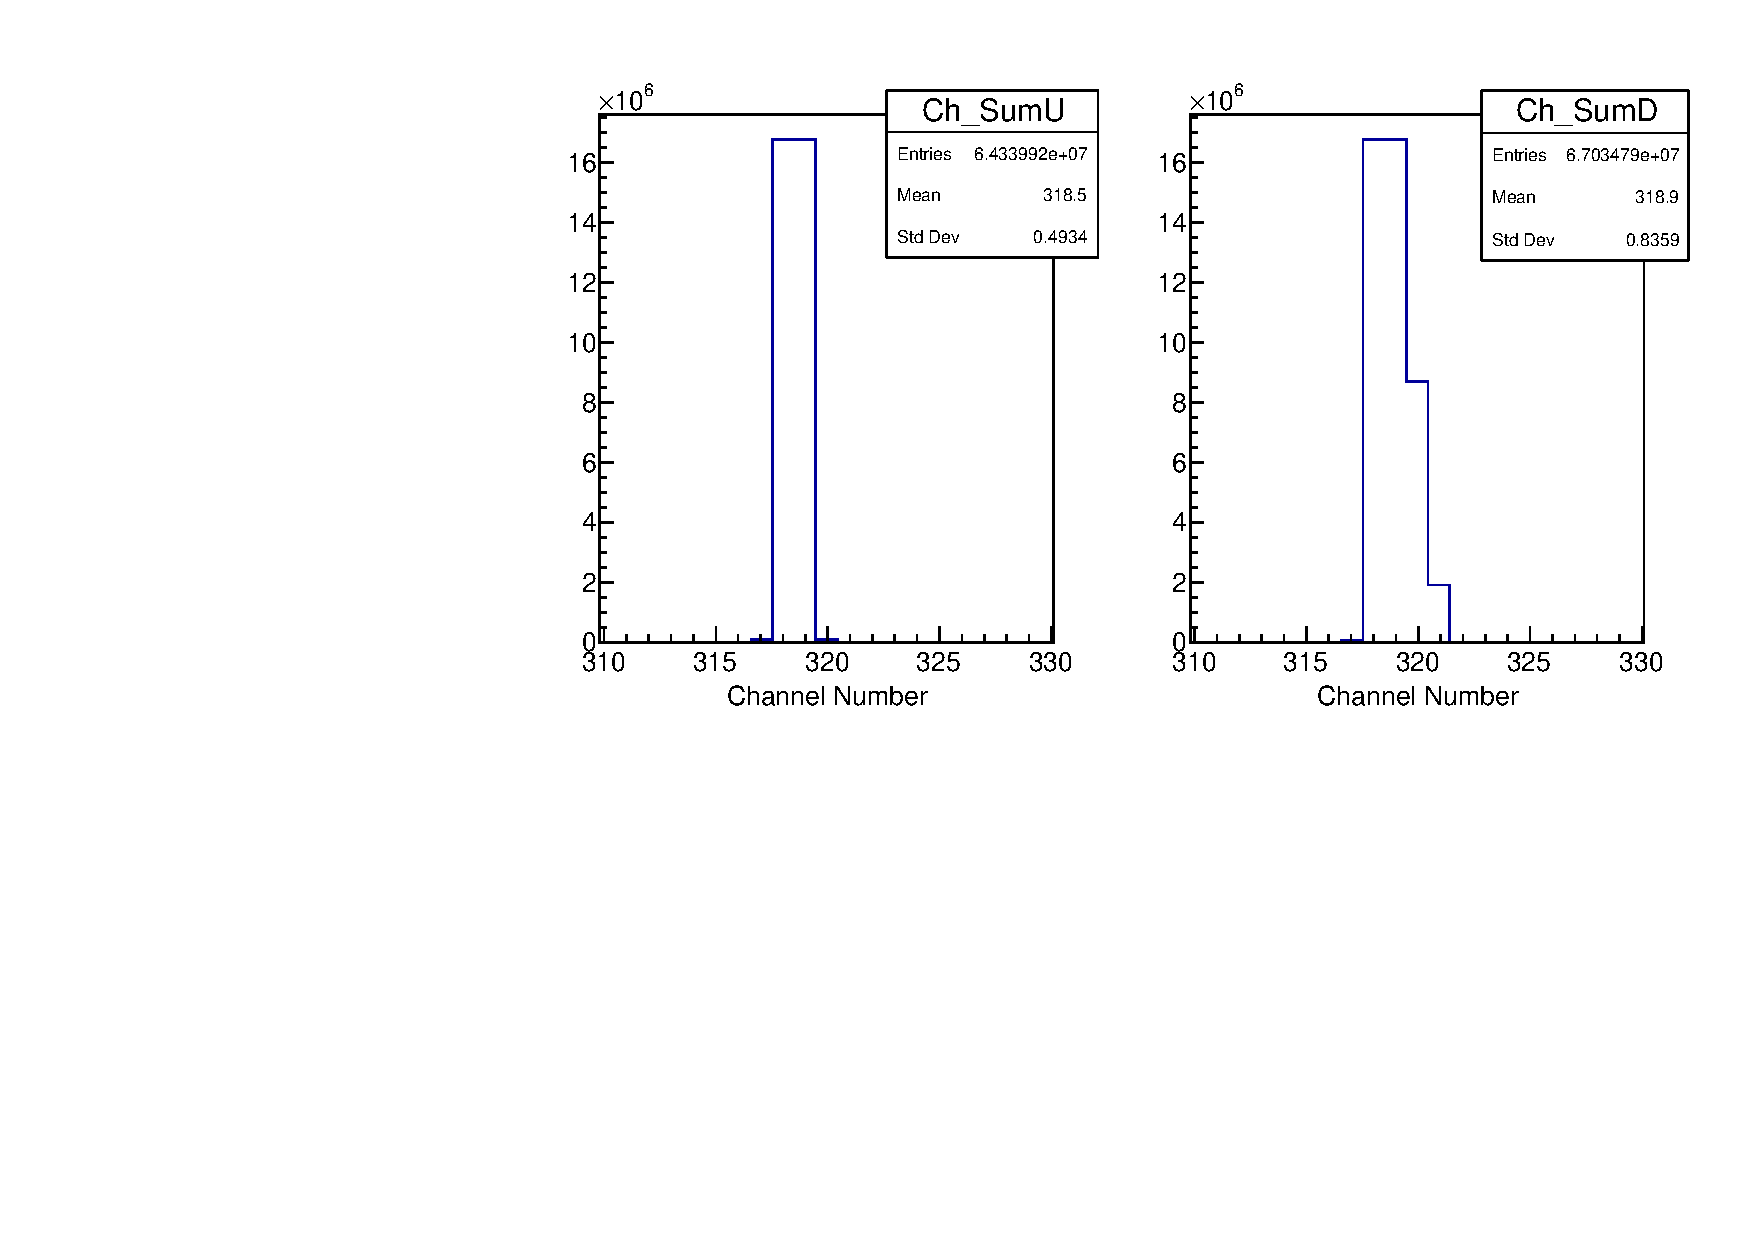
\includegraphics[width=0.7\textwidth, angle=0]{08-Performance/Kuno6mm.pdf}
    \caption{\label{fig:kuno} A plot showing the sum of the channel numbers for the clusters in each spacepoint for the upstream (left) and downstream (right) trackers. Kuno's conjecture that the sum is a constant is observed, with a small variation arising from the way fibre overlap is modelled in the Monte Carlo.}
  \end{figure}

  \begin{figure}[p]
    \centering
    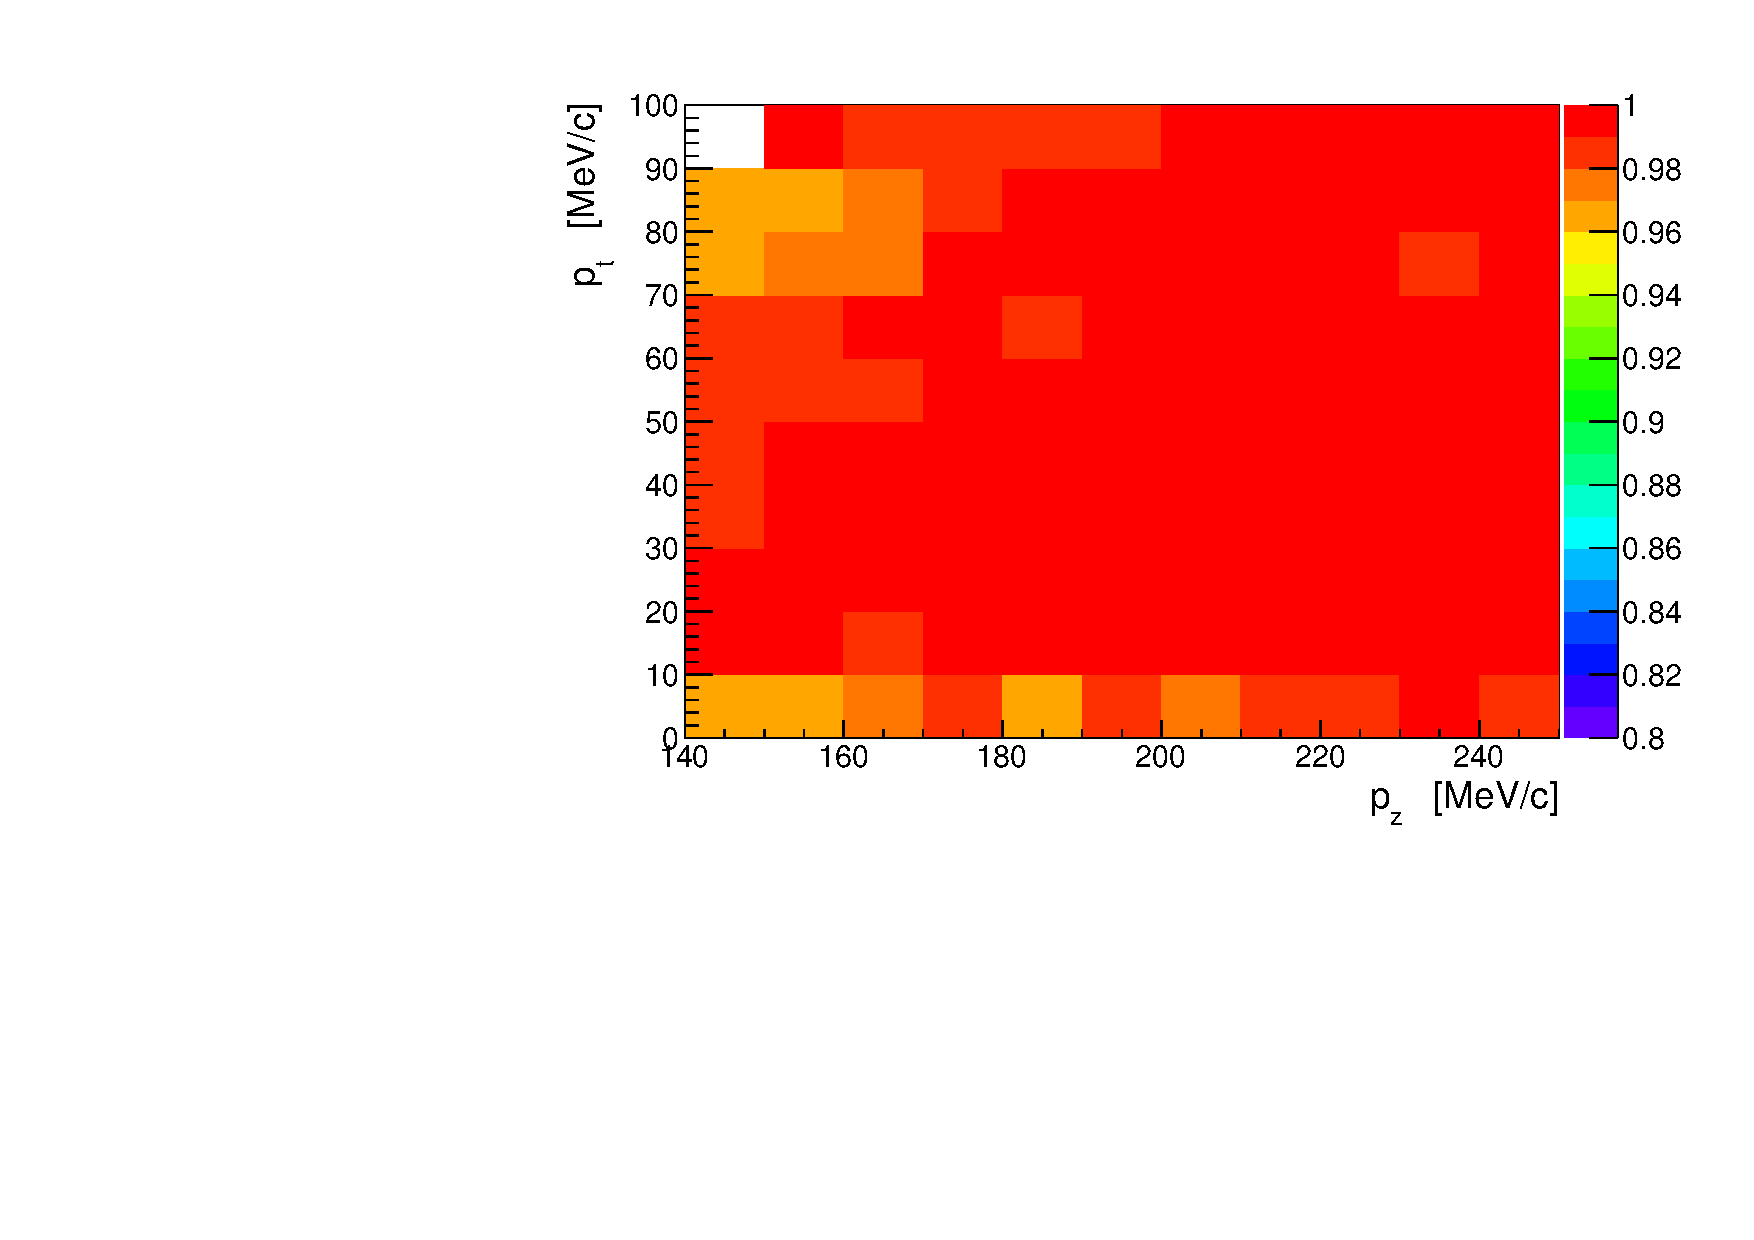
\includegraphics[width=0.495\textwidth, angle=0]{08-Performance/upstream_track_efficiency.pdf}
    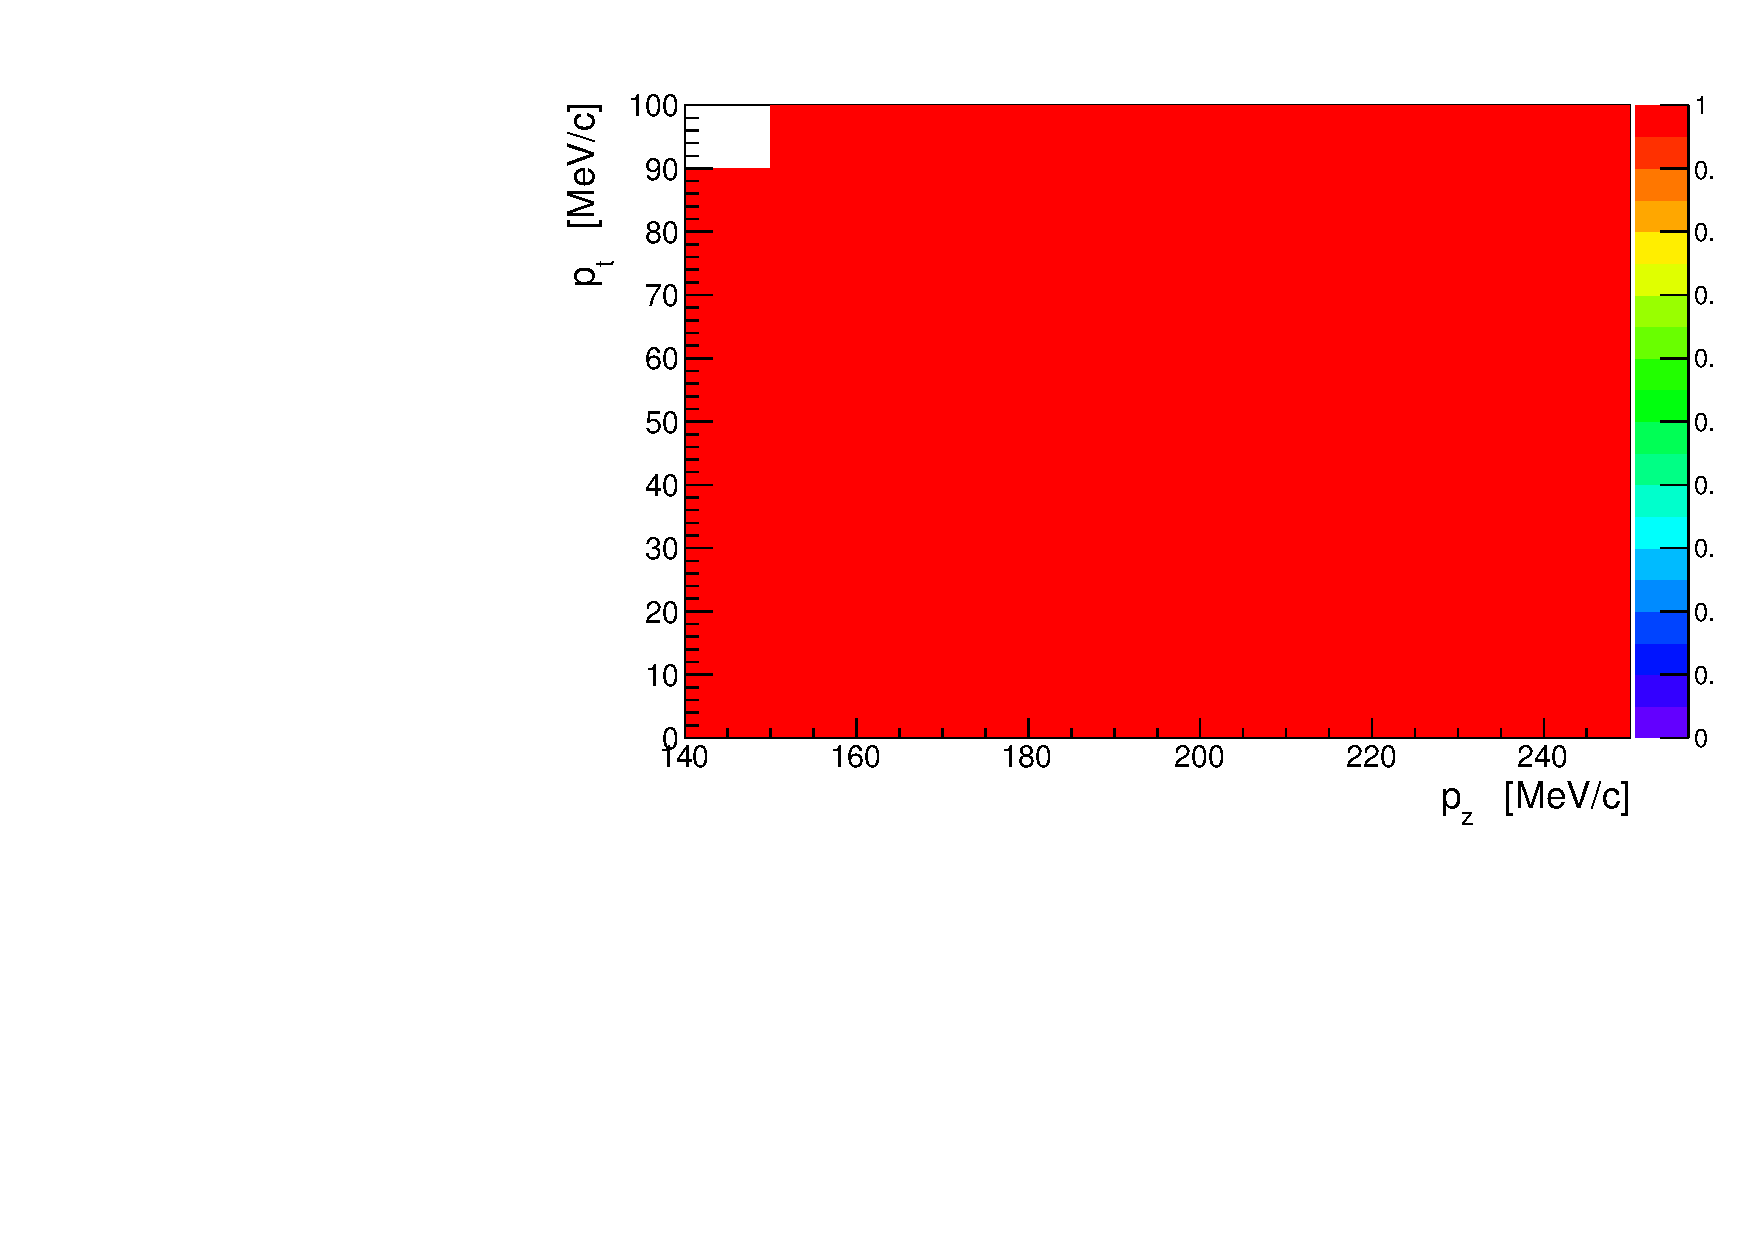
\includegraphics[width=0.495\textwidth, angle=0]{08-Performance/downstream_track_efficiency.pdf}\\
    \caption{\label{fig:track_efficiency} The efficiency of reconstructing tracks in the upstream (left) and downstream (right) trackers as a function of the simulated longitudinal and transverse momentum. The white area in the top left of the plot indicates events which fall outside of the $p_t/p_z$ ratio cut.}
  \end{figure}

%   \begin{figure}[p]
%     \centering
%     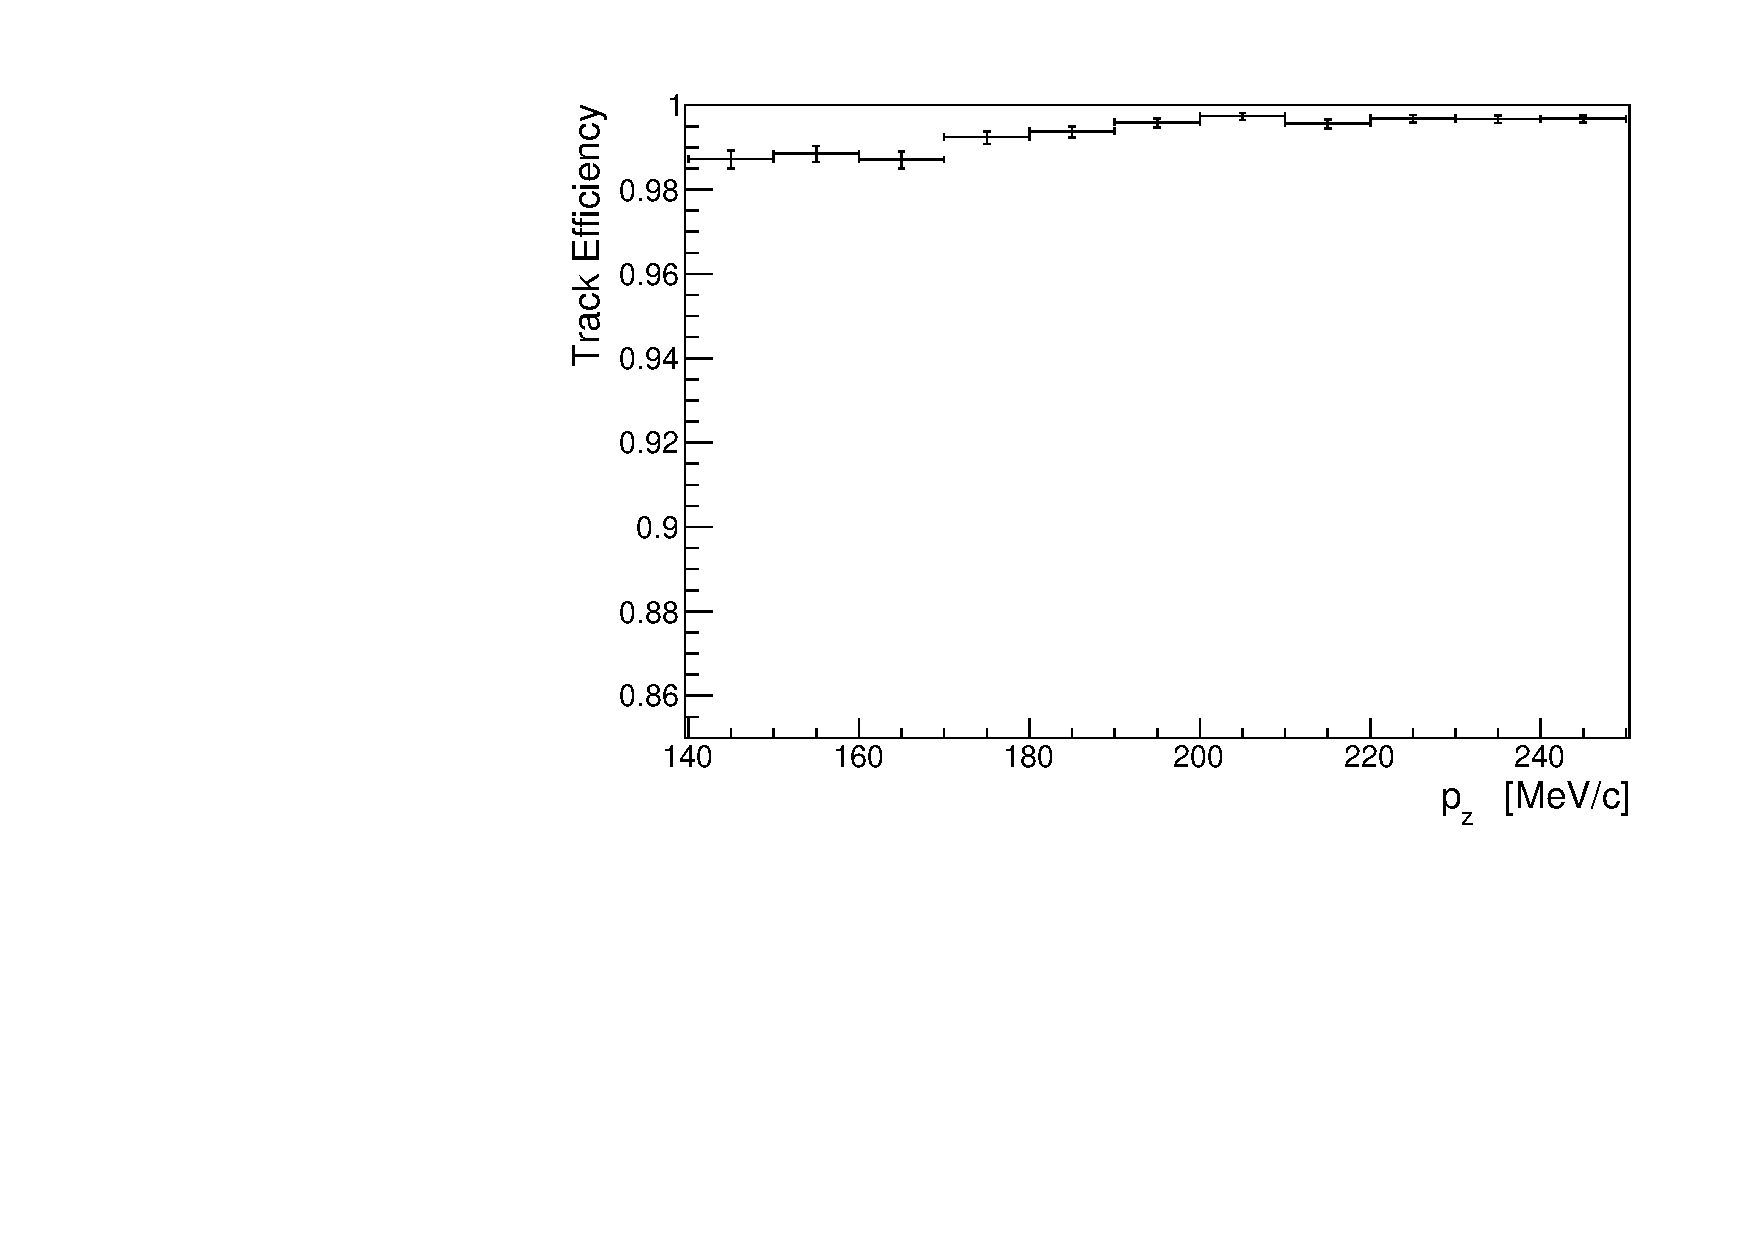
\includegraphics[width=0.45\textwidth, angle=0]{08-Performance/upstream_pz_track_efficiency.pdf}
%     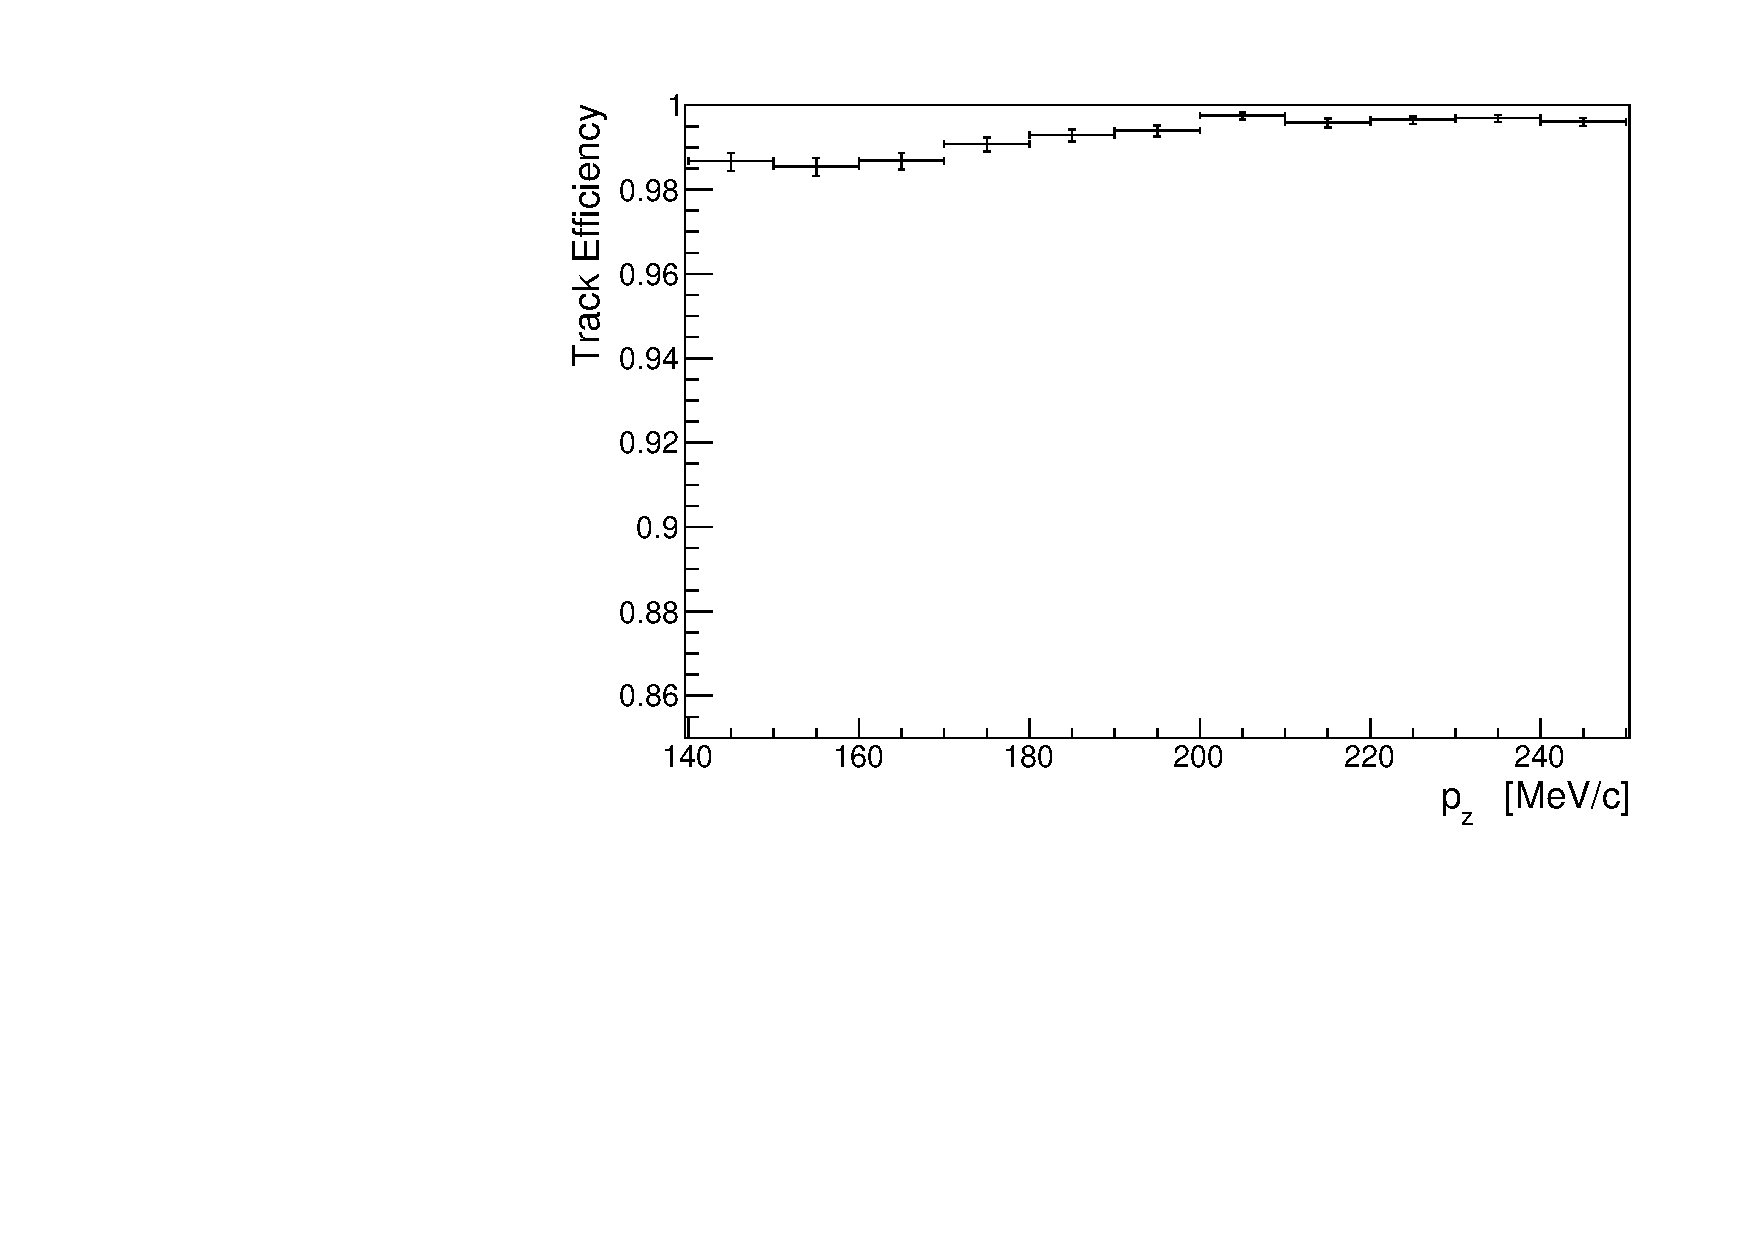
\includegraphics[width=0.45\textwidth, angle=0]{08-Performance/downstream_pz_track_efficiency.pdf}\\
%     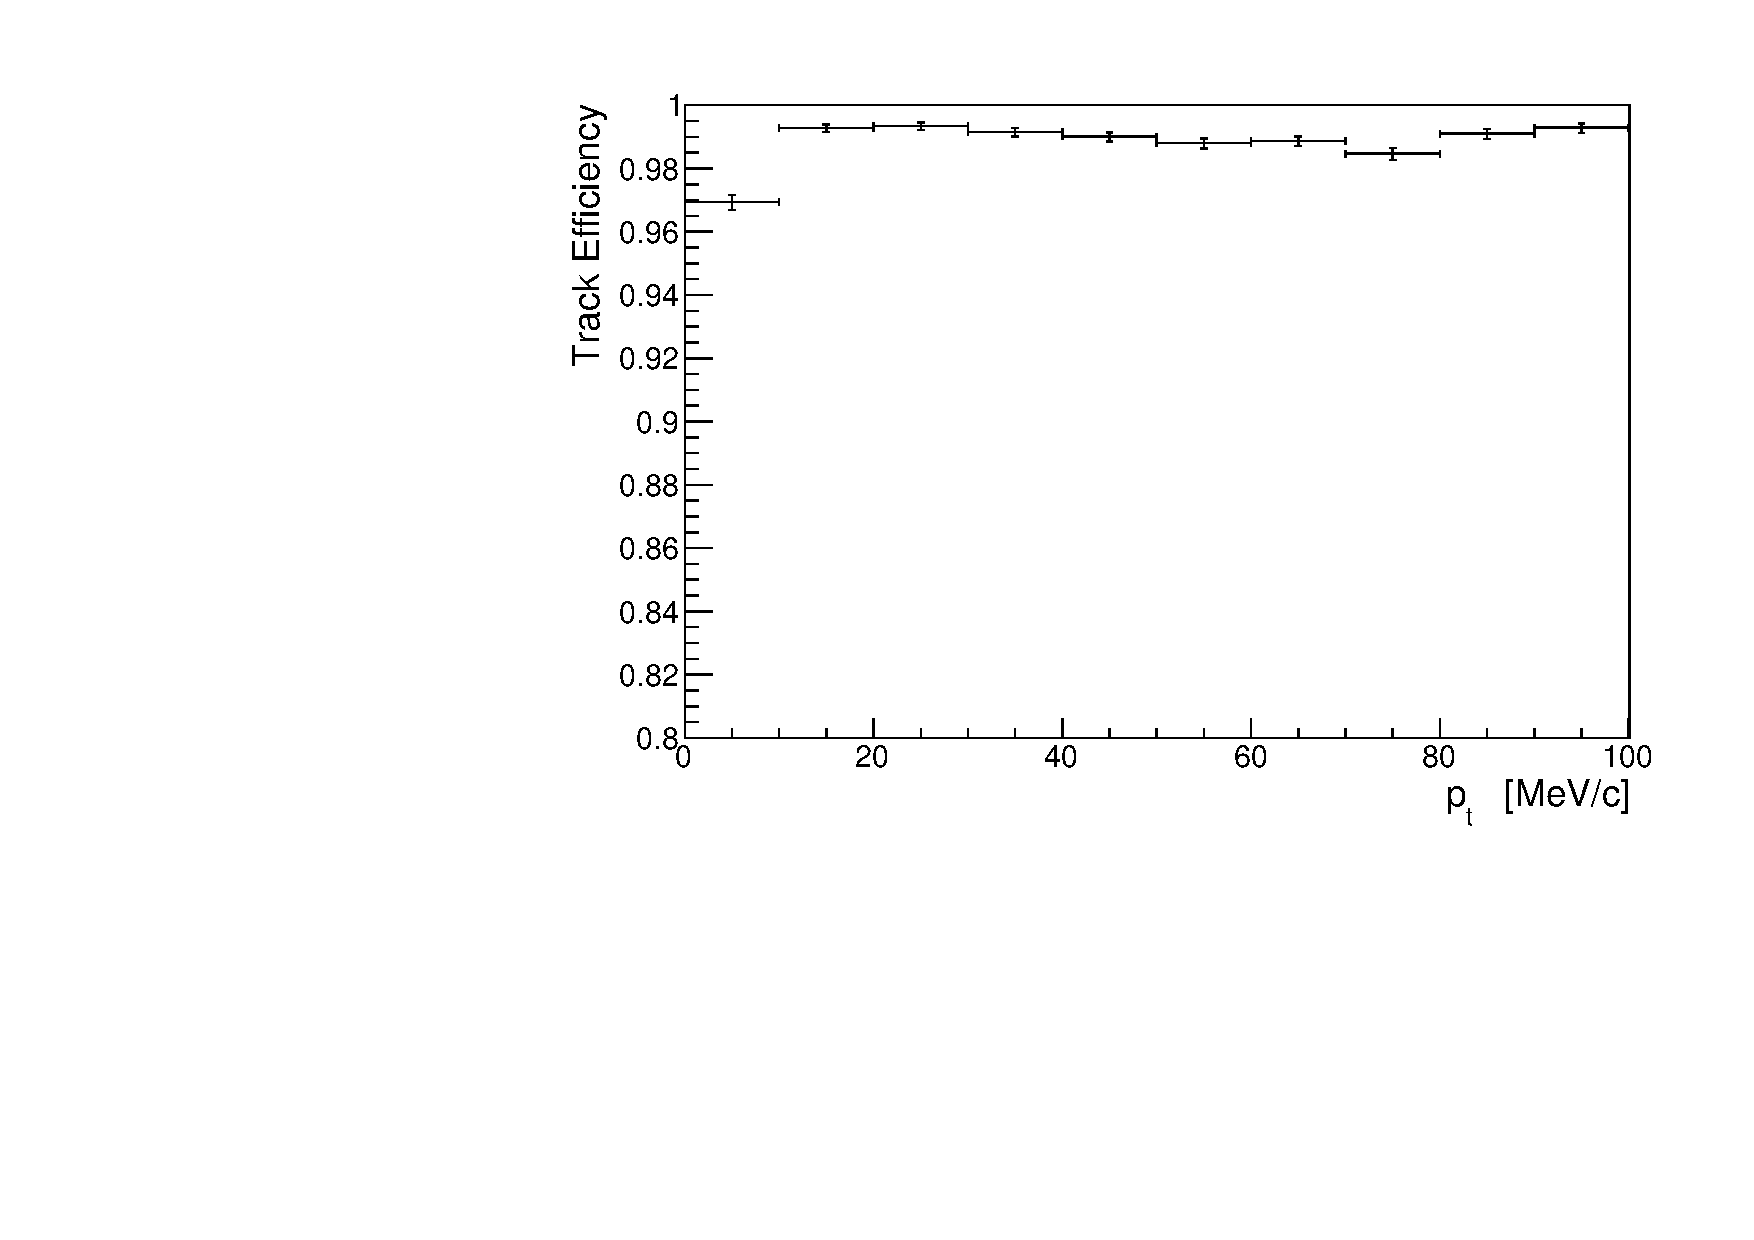
\includegraphics[width=0.45\textwidth, angle=0]{08-Performance/upstream_pt_track_efficiency.pdf}
%     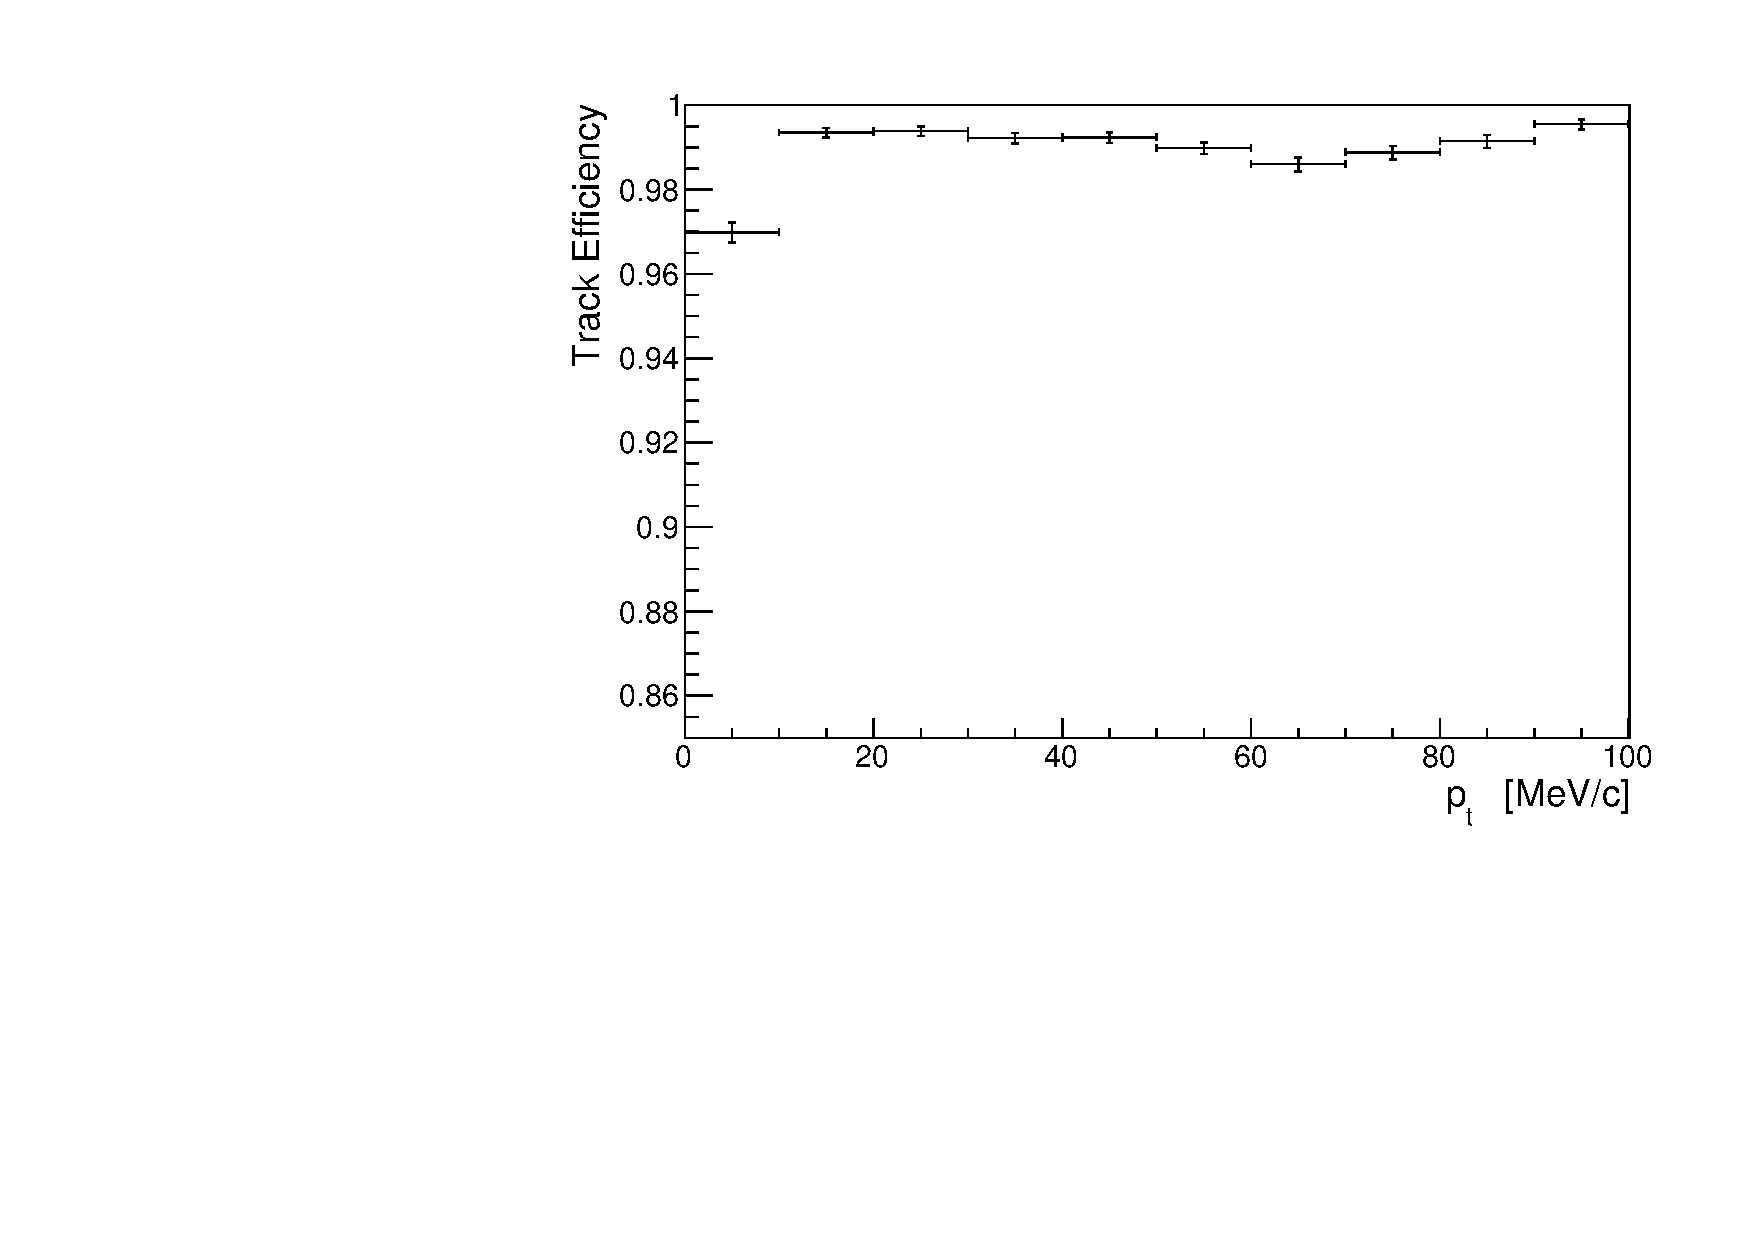
\includegraphics[width=0.45\textwidth, angle=0]{08-Performance/downstream_pt_track_efficiency.pdf}
%     \caption{\label{fig:track_efficiency} The efficiency of reconstructing tracks in the upstream (left) and downstream (right) trackers as a function of the simulated longitudinal (top) and transverse (bottom) momentum.}
%   \end{figure}
  
%   \begin{figure}[p]
%     \centering
%     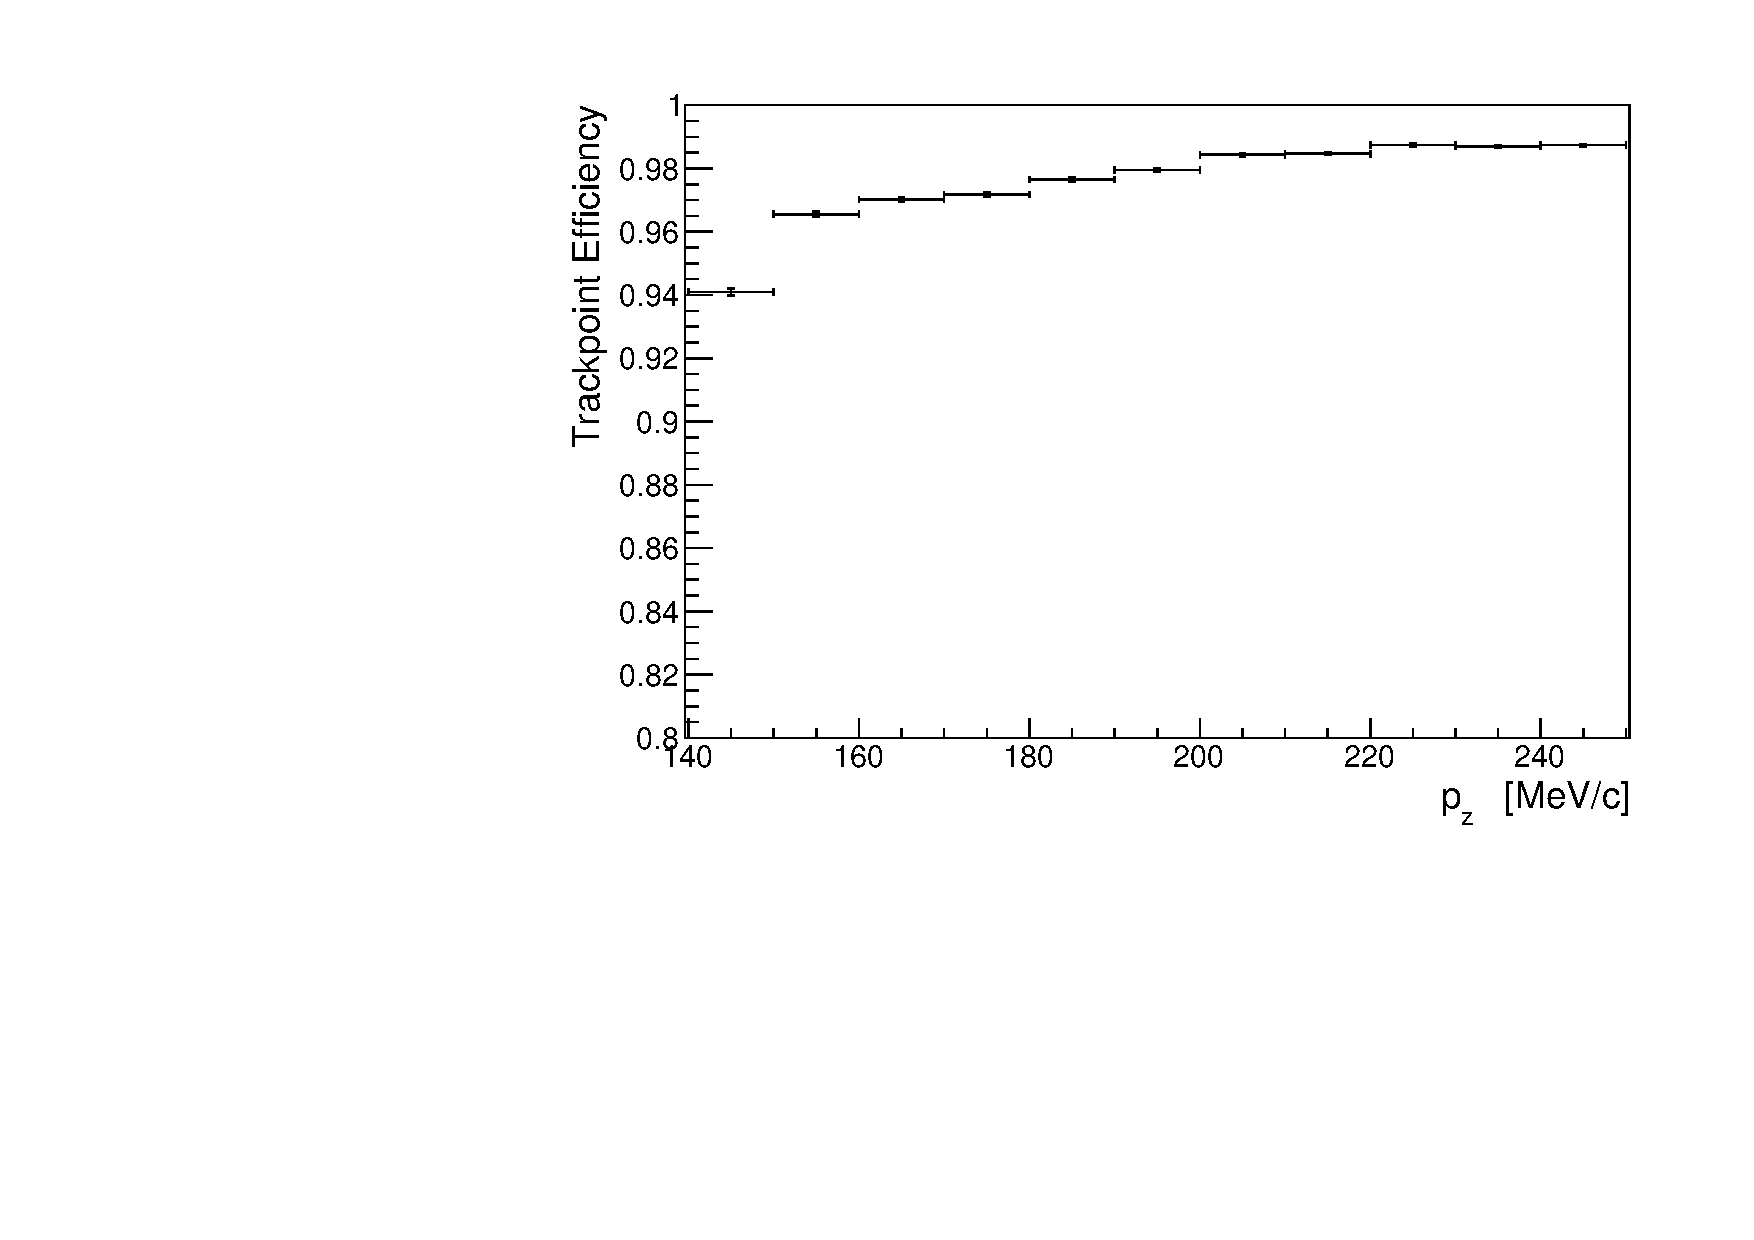
\includegraphics[width=0.45\textwidth, angle=0]{08-Performance/upstream_pz_tp_efficiency.pdf}
%     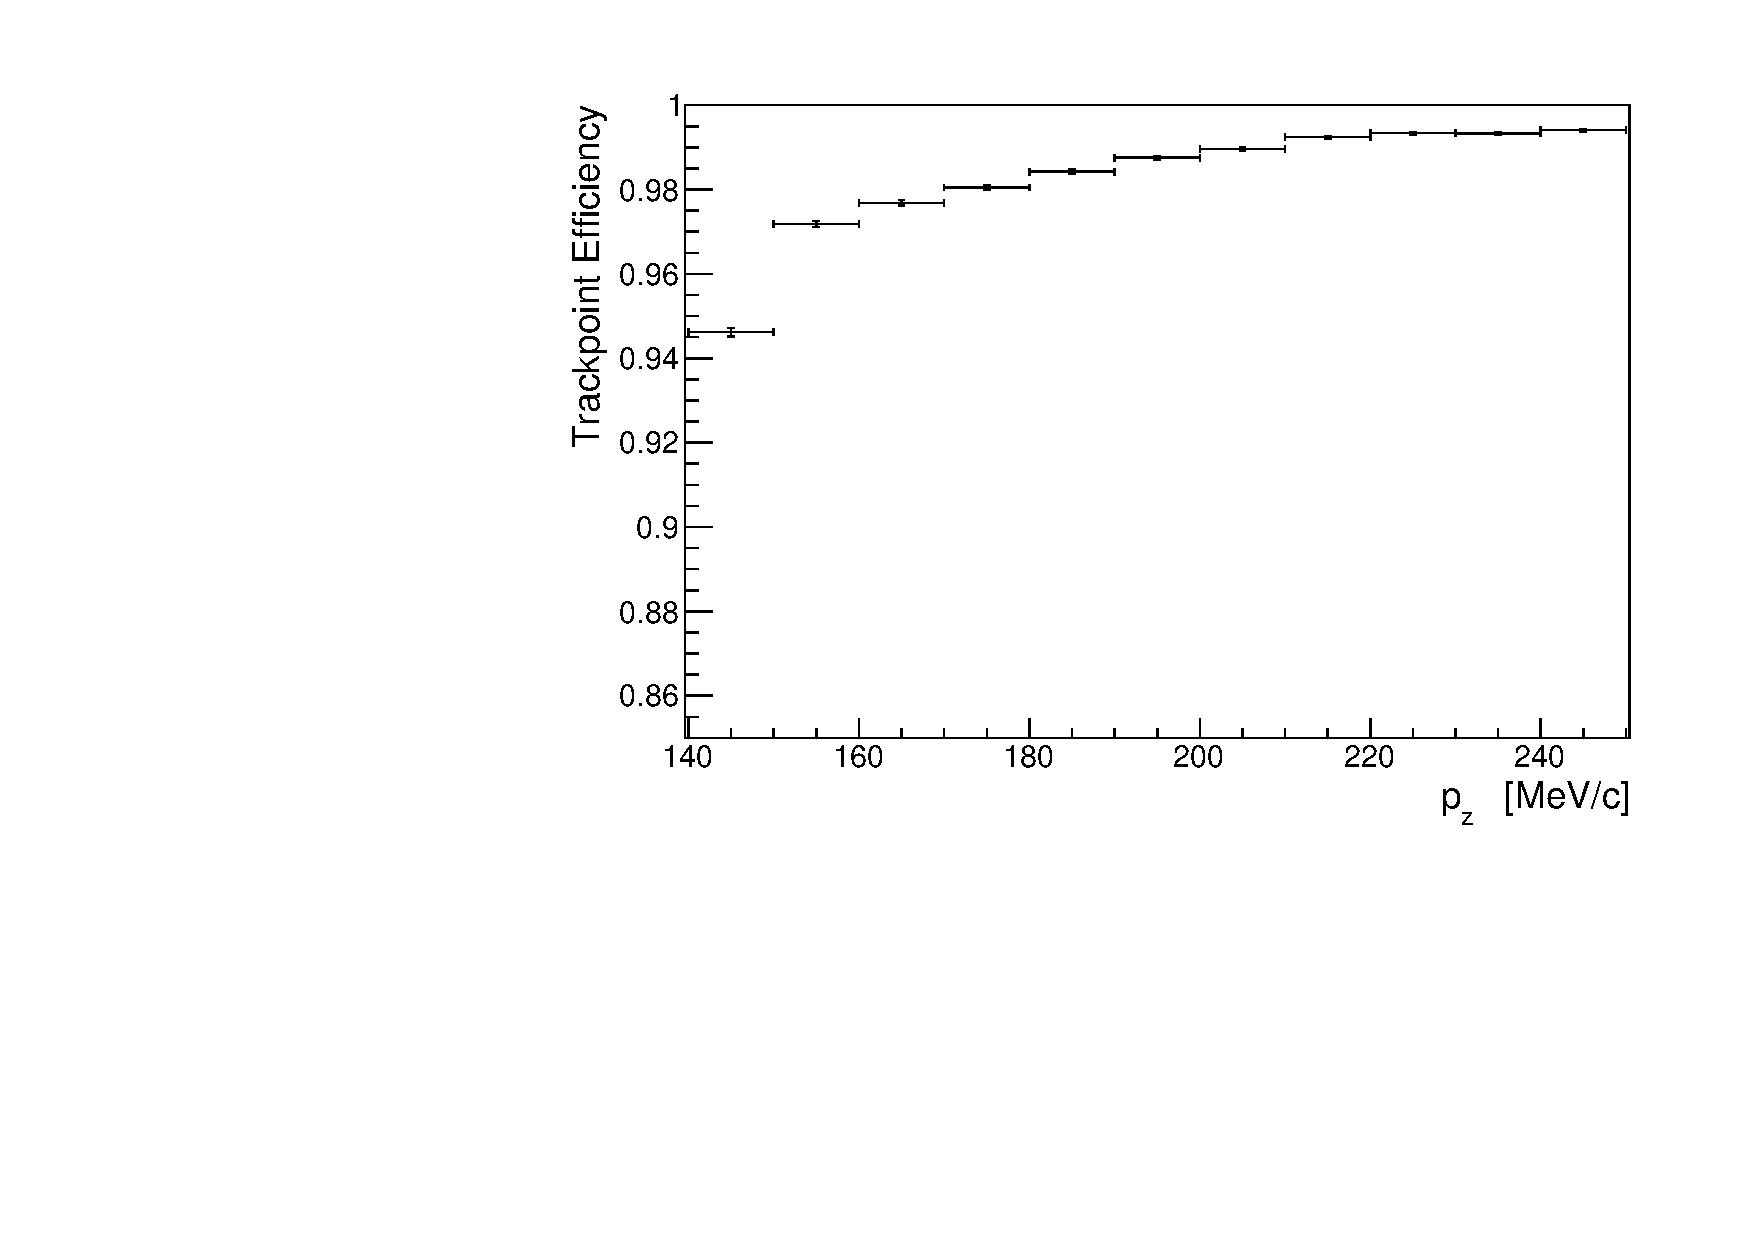
\includegraphics[width=0.45\textwidth, angle=0]{08-Performance/downstream_pz_tp_efficiency.pdf}\\
%     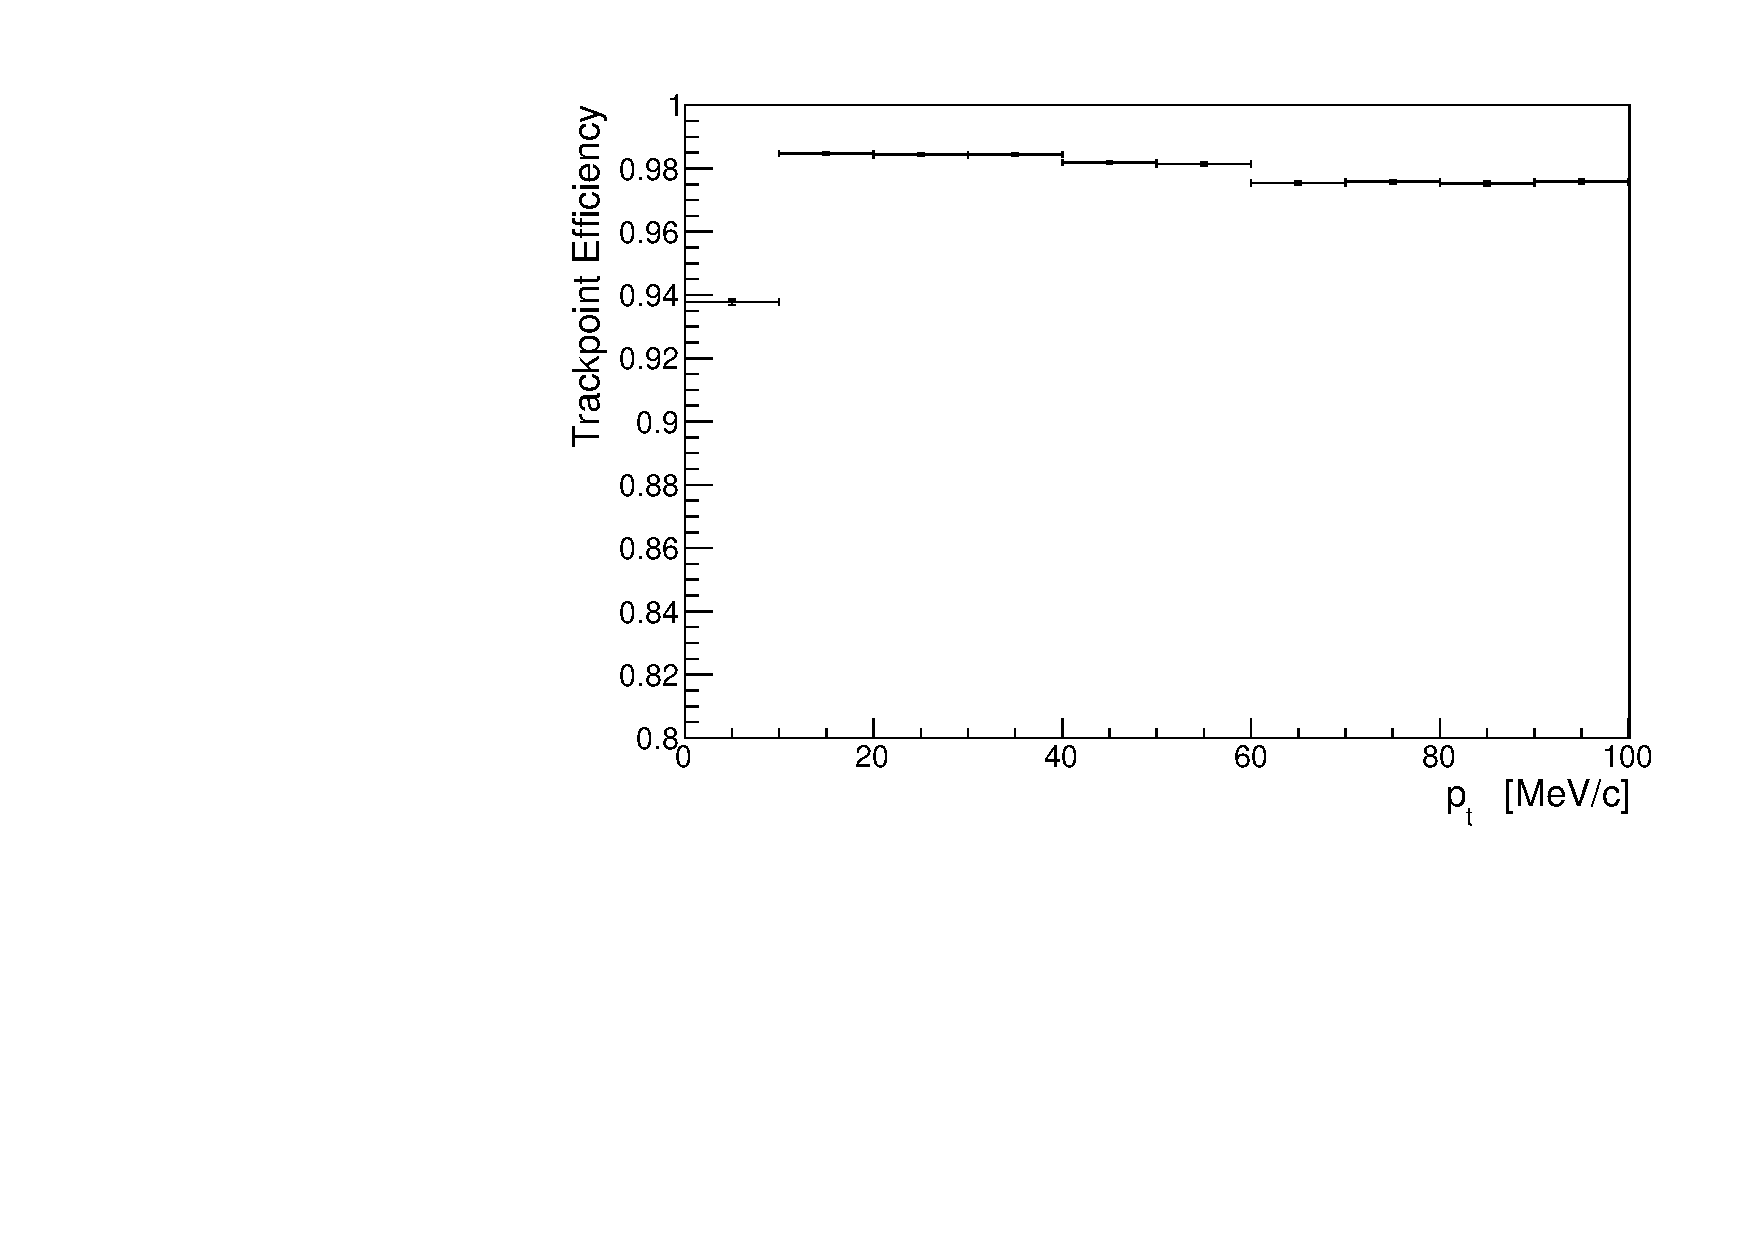
\includegraphics[width=0.45\textwidth, angle=0]{08-Performance/upstream_pt_tp_efficiency.pdf}
%     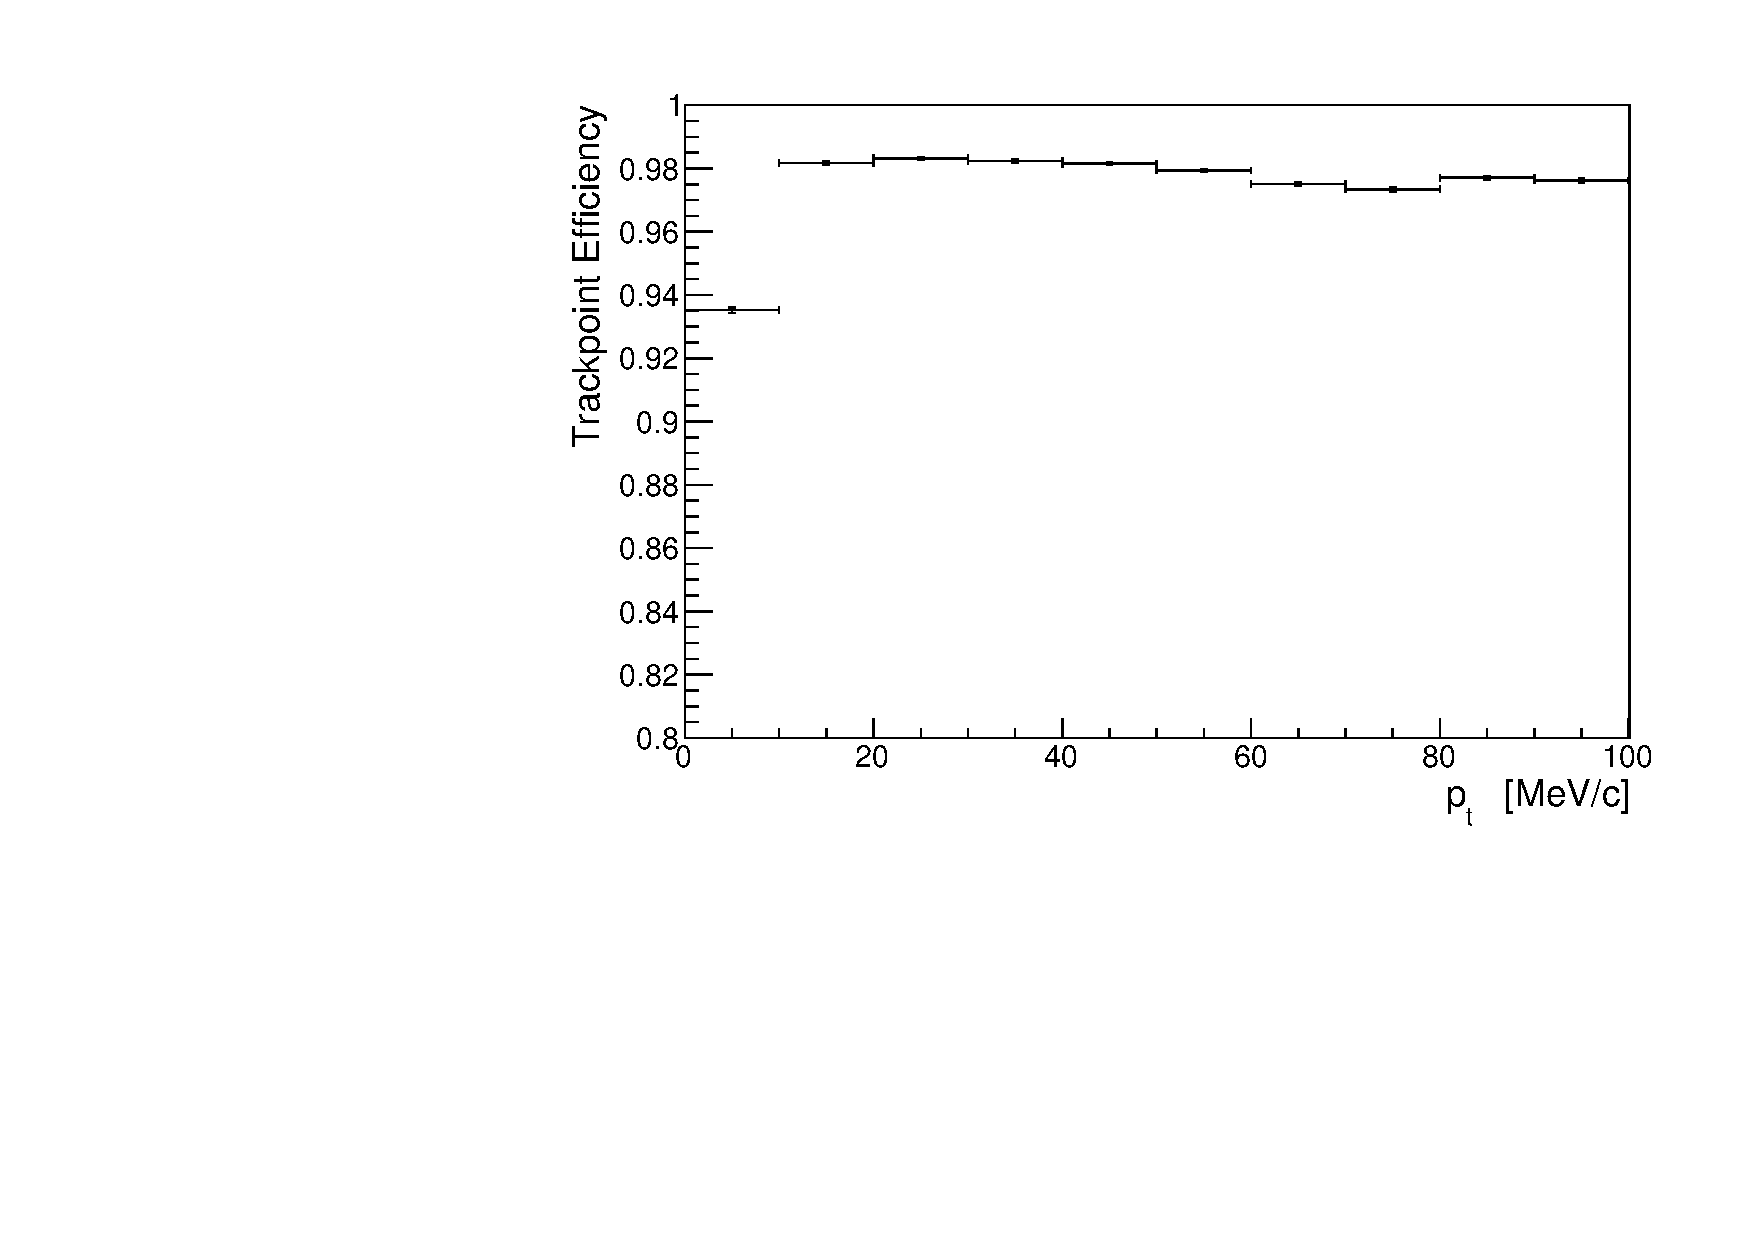
\includegraphics[width=0.45\textwidth, angle=0]{08-Performance/downstream_pt_tp_efficiency.pdf}
%     \caption{\label{fig:tp_efficiency} The efficiency of reconstructing trackpoints in the upstream (left) and downstream (right) trackers as a function of the simulated longitudinal (top) and transverse (bottom) momentum.}
%   \end{figure}
  
  \begin{figure}[p]
   \centering
    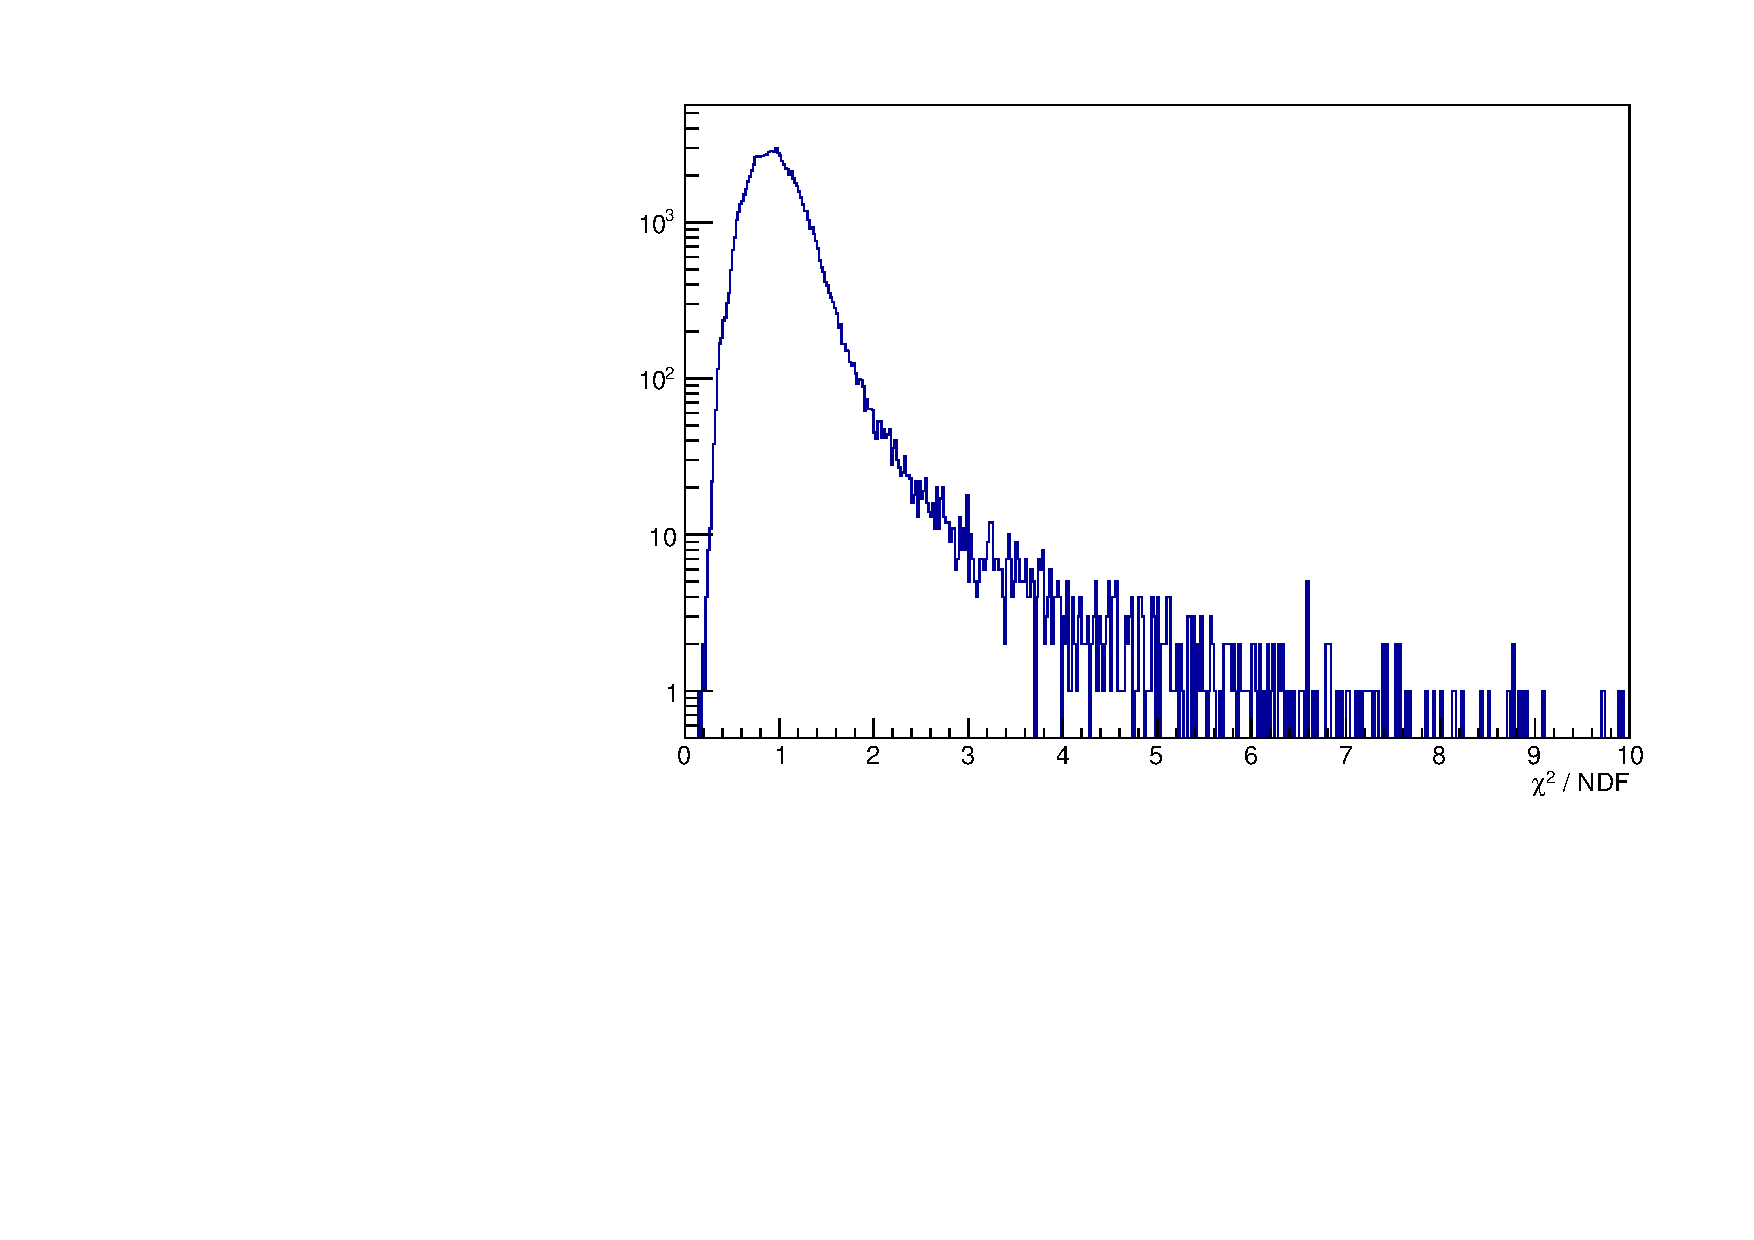
\includegraphics[width=0.49\textwidth, angle=0]{08-Performance/chi_squared_ndf_up.pdf}
    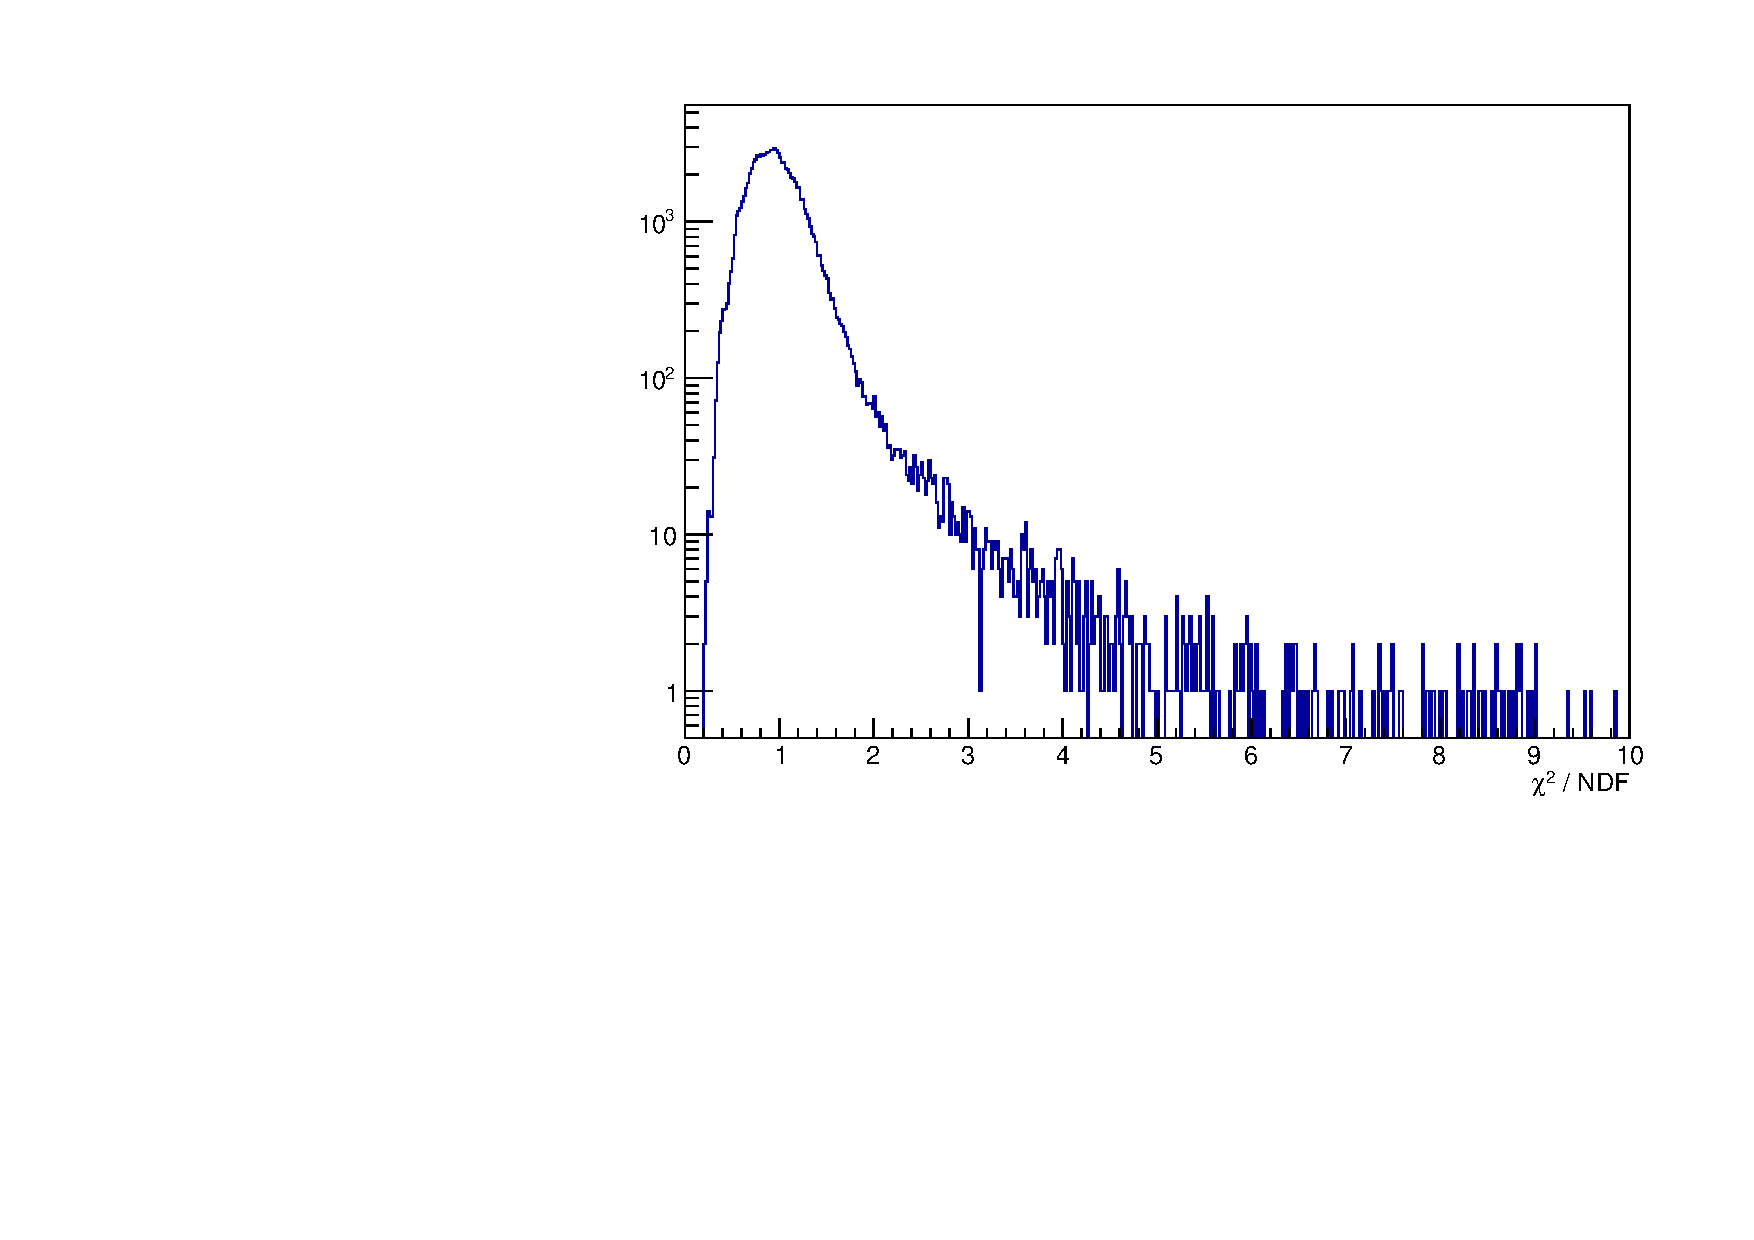
\includegraphics[width=0.49\textwidth, angle=0]{08-Performance/chi_squared_ndf_down.pdf}
   \caption{\label{fig:track_chisq} The $\chi^2$ per degree of freedom in the upstream (left) and downstream (right) trackers.}
  \end{figure}
  
  \begin{figure}[p]
    \begin{center}
      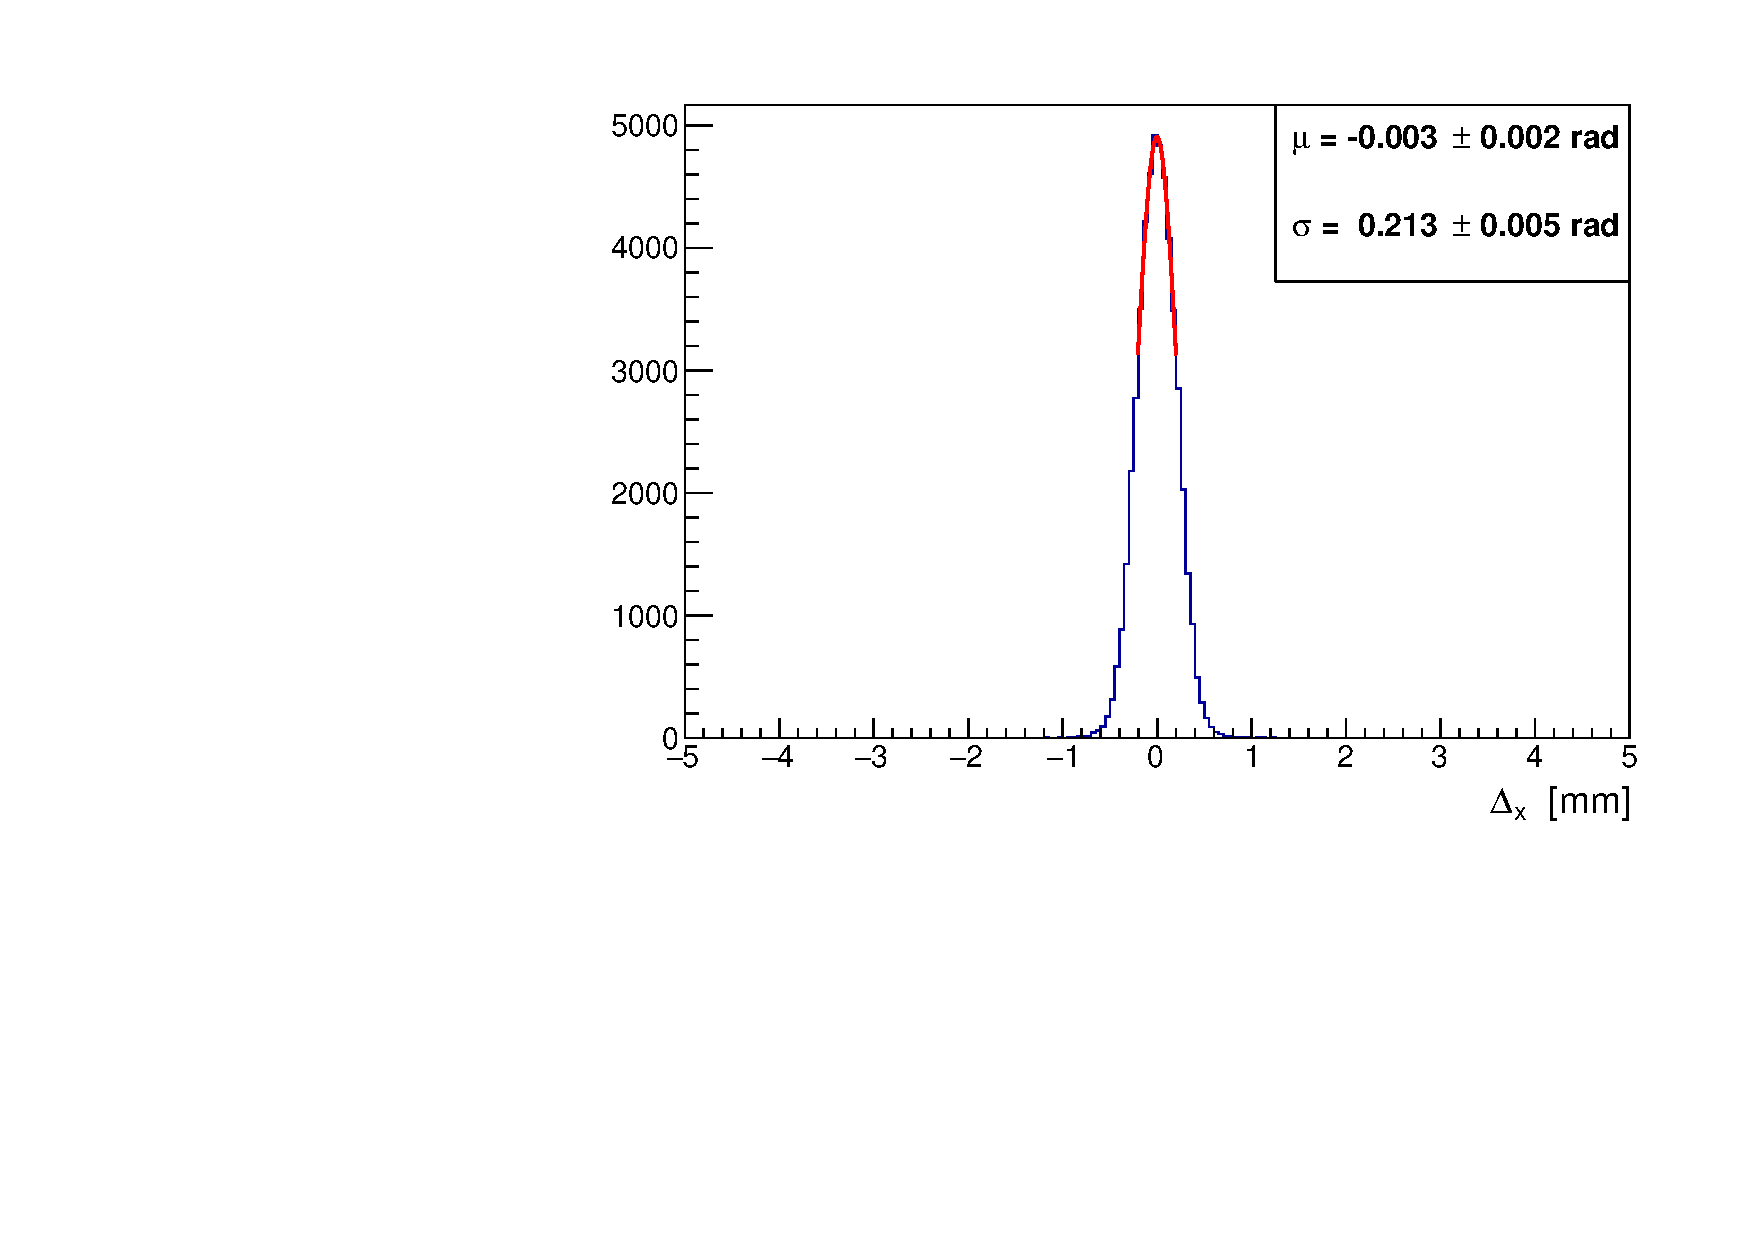
\includegraphics[width=0.49\textwidth, angle=0]{08-Performance/upstream_x_residual.pdf}
      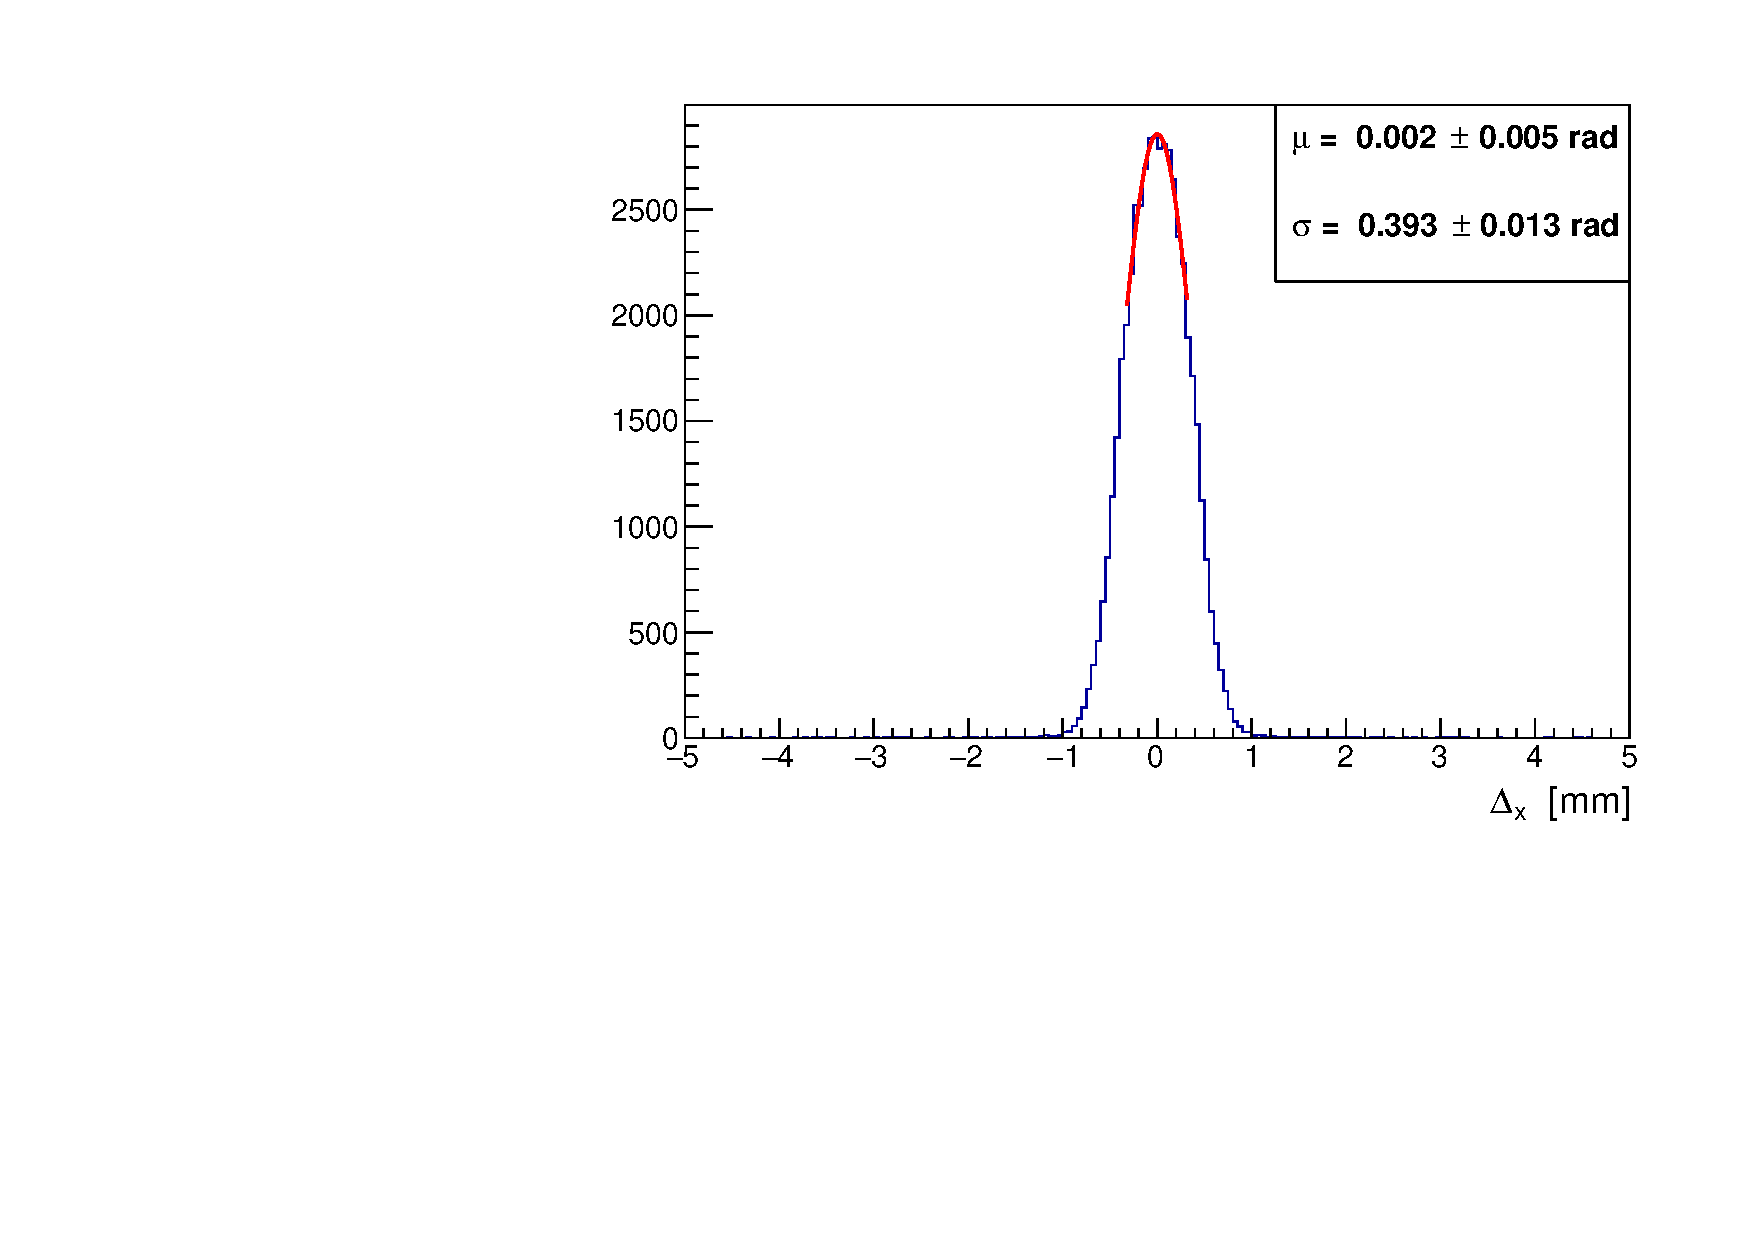
\includegraphics[width=0.49\textwidth, angle=0]{08-Performance/downstream_x_residual.pdf}
      \caption{\label{fig:XResidKalman} The $x$ residuals of the upstream (left) and downstream (right) trackers.}
    \end{center}
  \end{figure}
  
    \begin{figure}[p]
    \begin{center}
      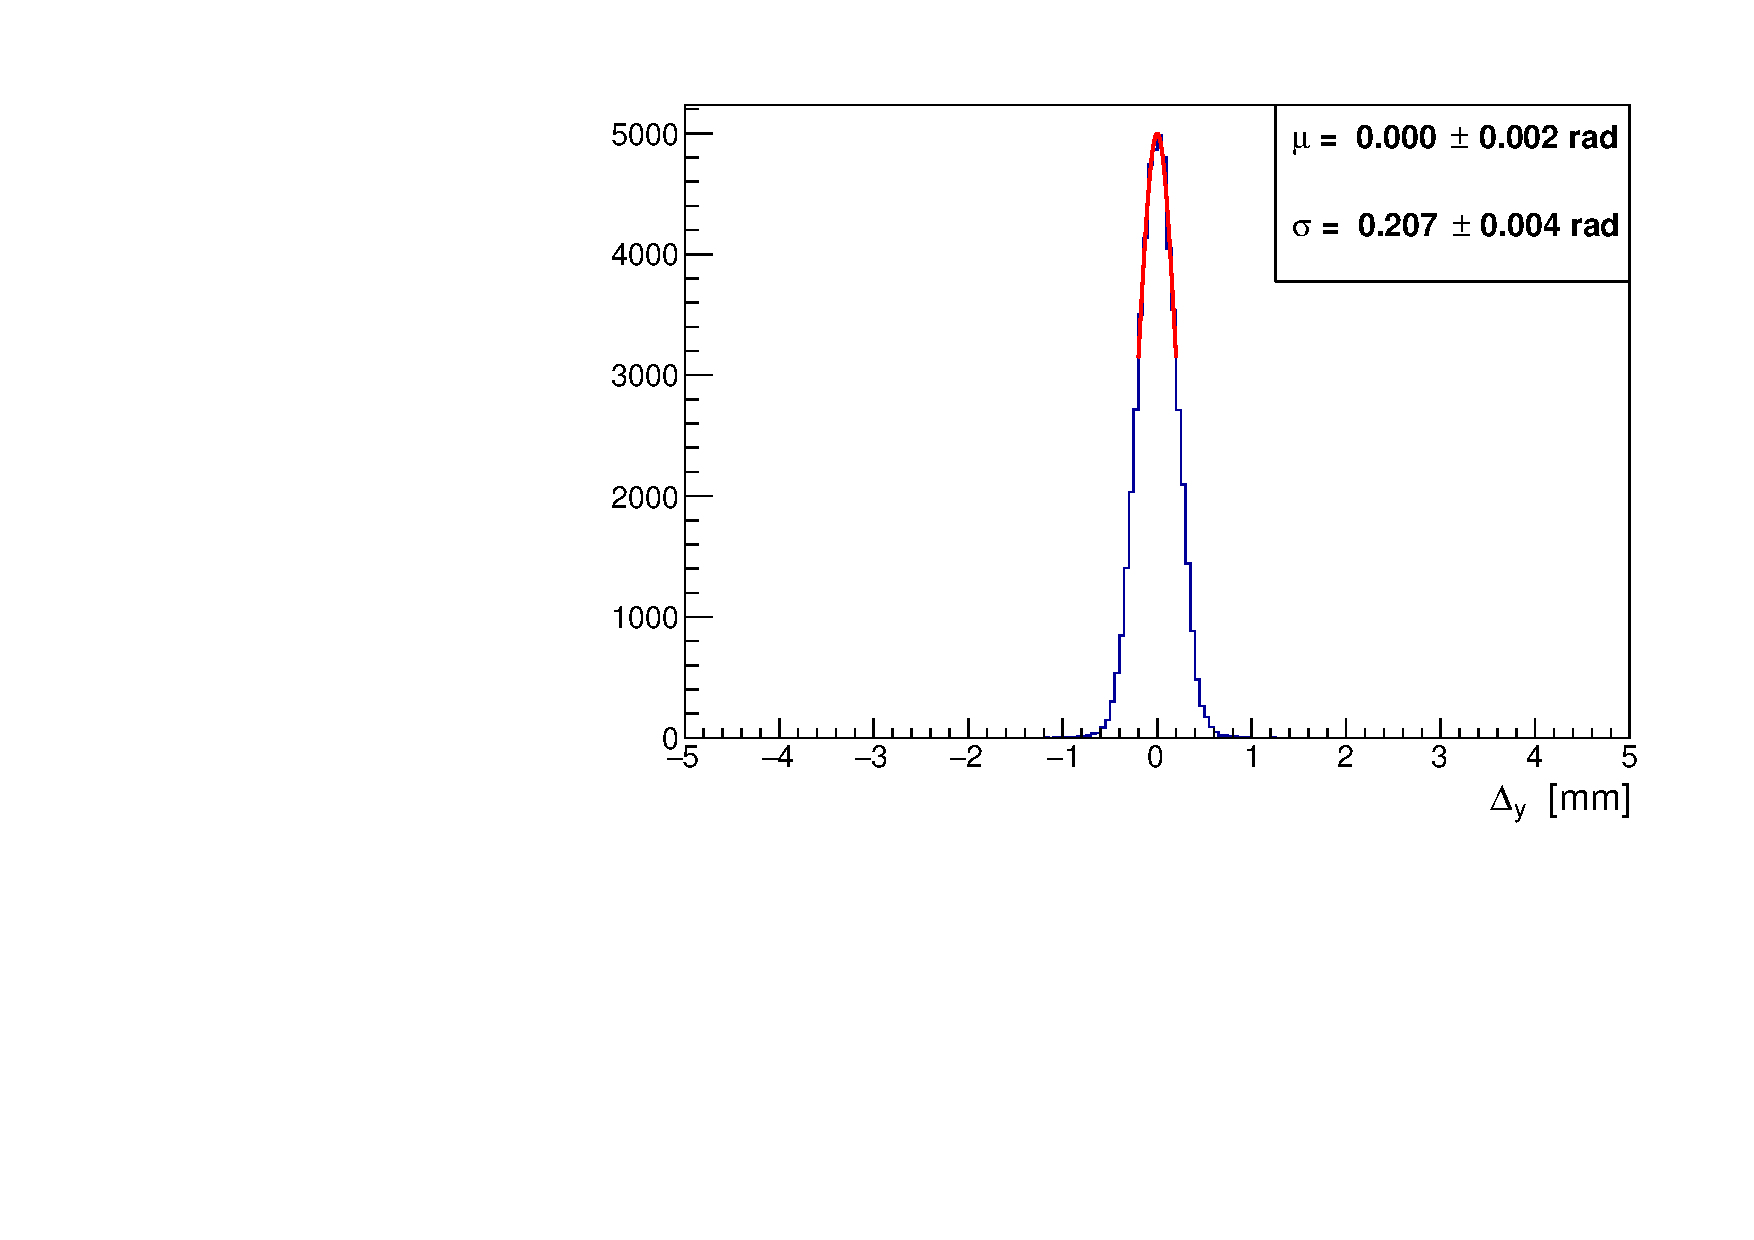
\includegraphics[width=0.49\textwidth, angle=0]{08-Performance/upstream_y_residual.pdf}
      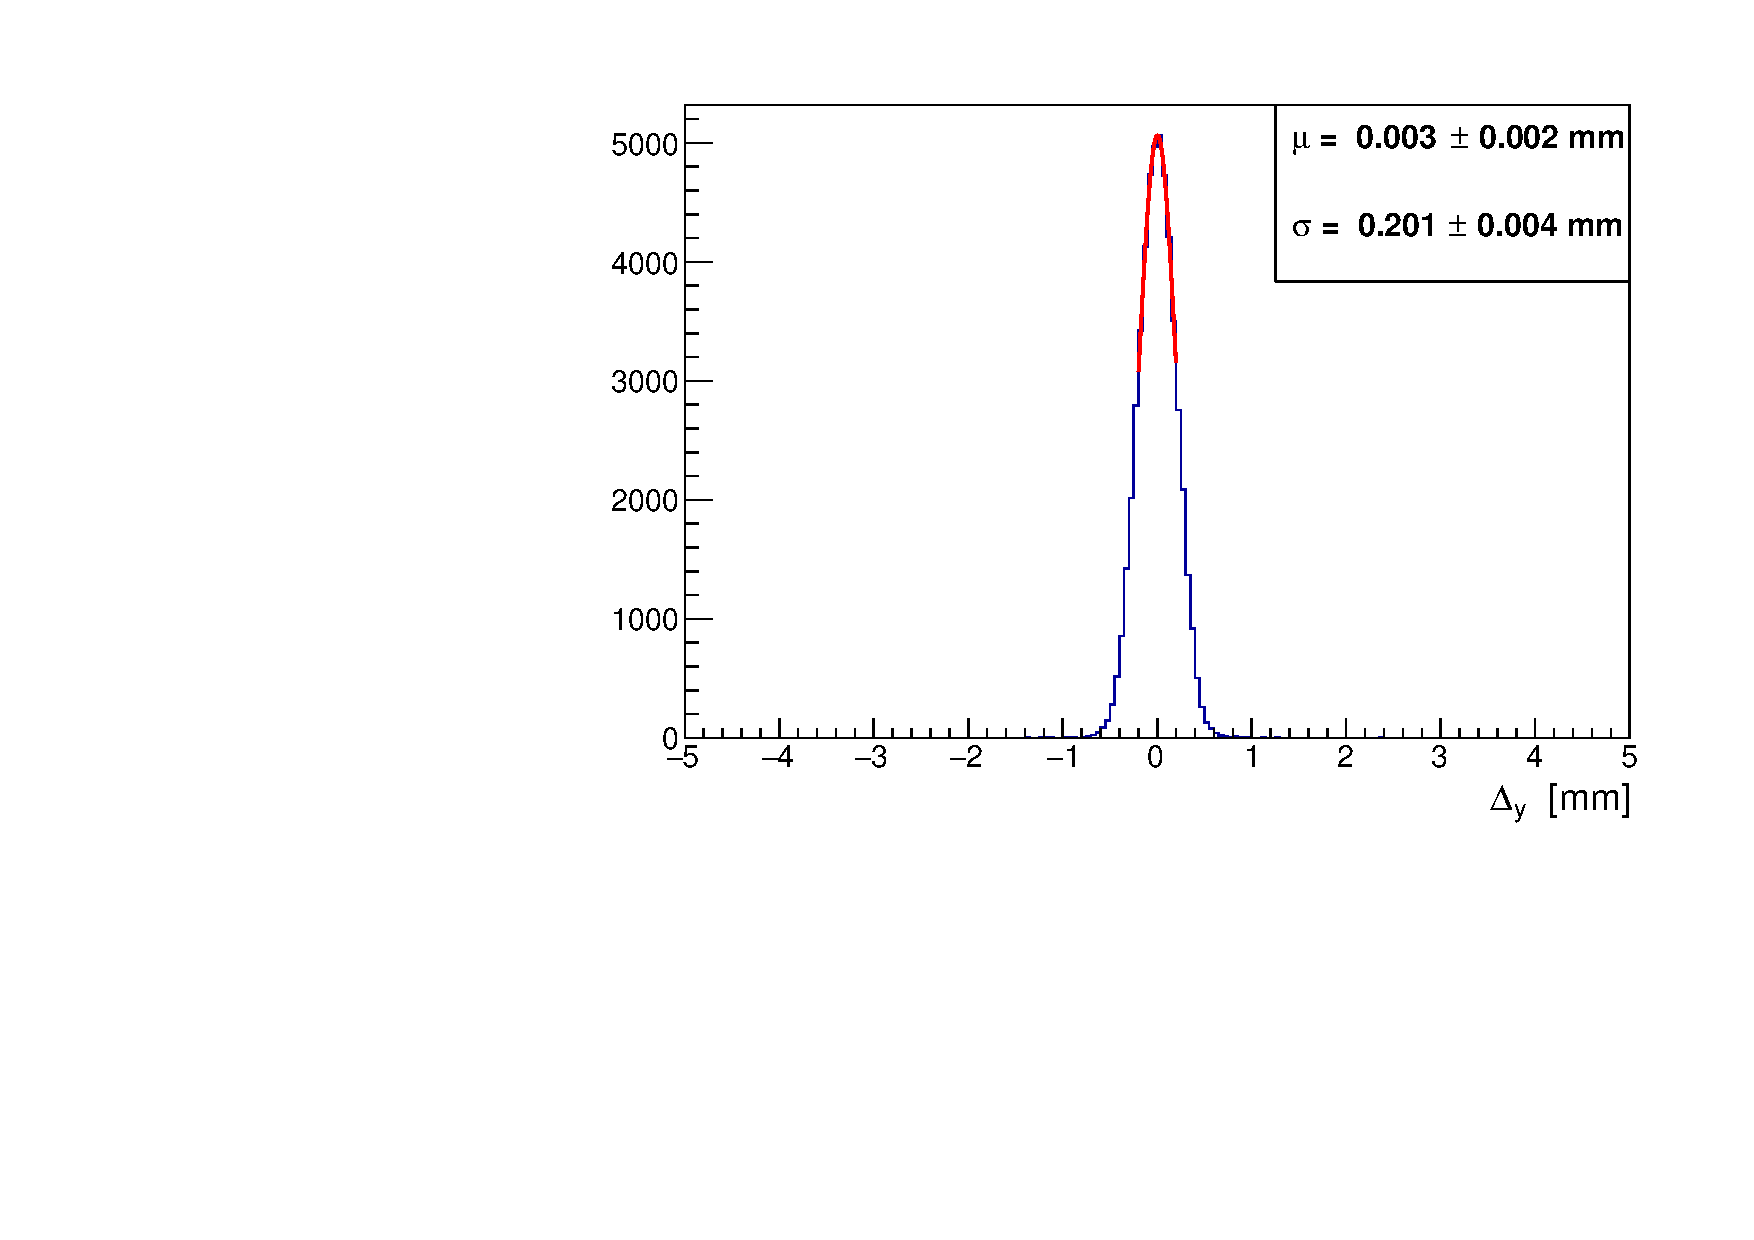
\includegraphics[width=0.49\textwidth, angle=0]{08-Performance/downstream_y_residual.pdf}
      \caption{\label{fig:YResidKalman} The $y$ residuals of the upstream (left) and downstream (right) trackers.}
    \end{center}
  \end{figure} 
  
  \begin{figure}[p]
    \begin{center}
      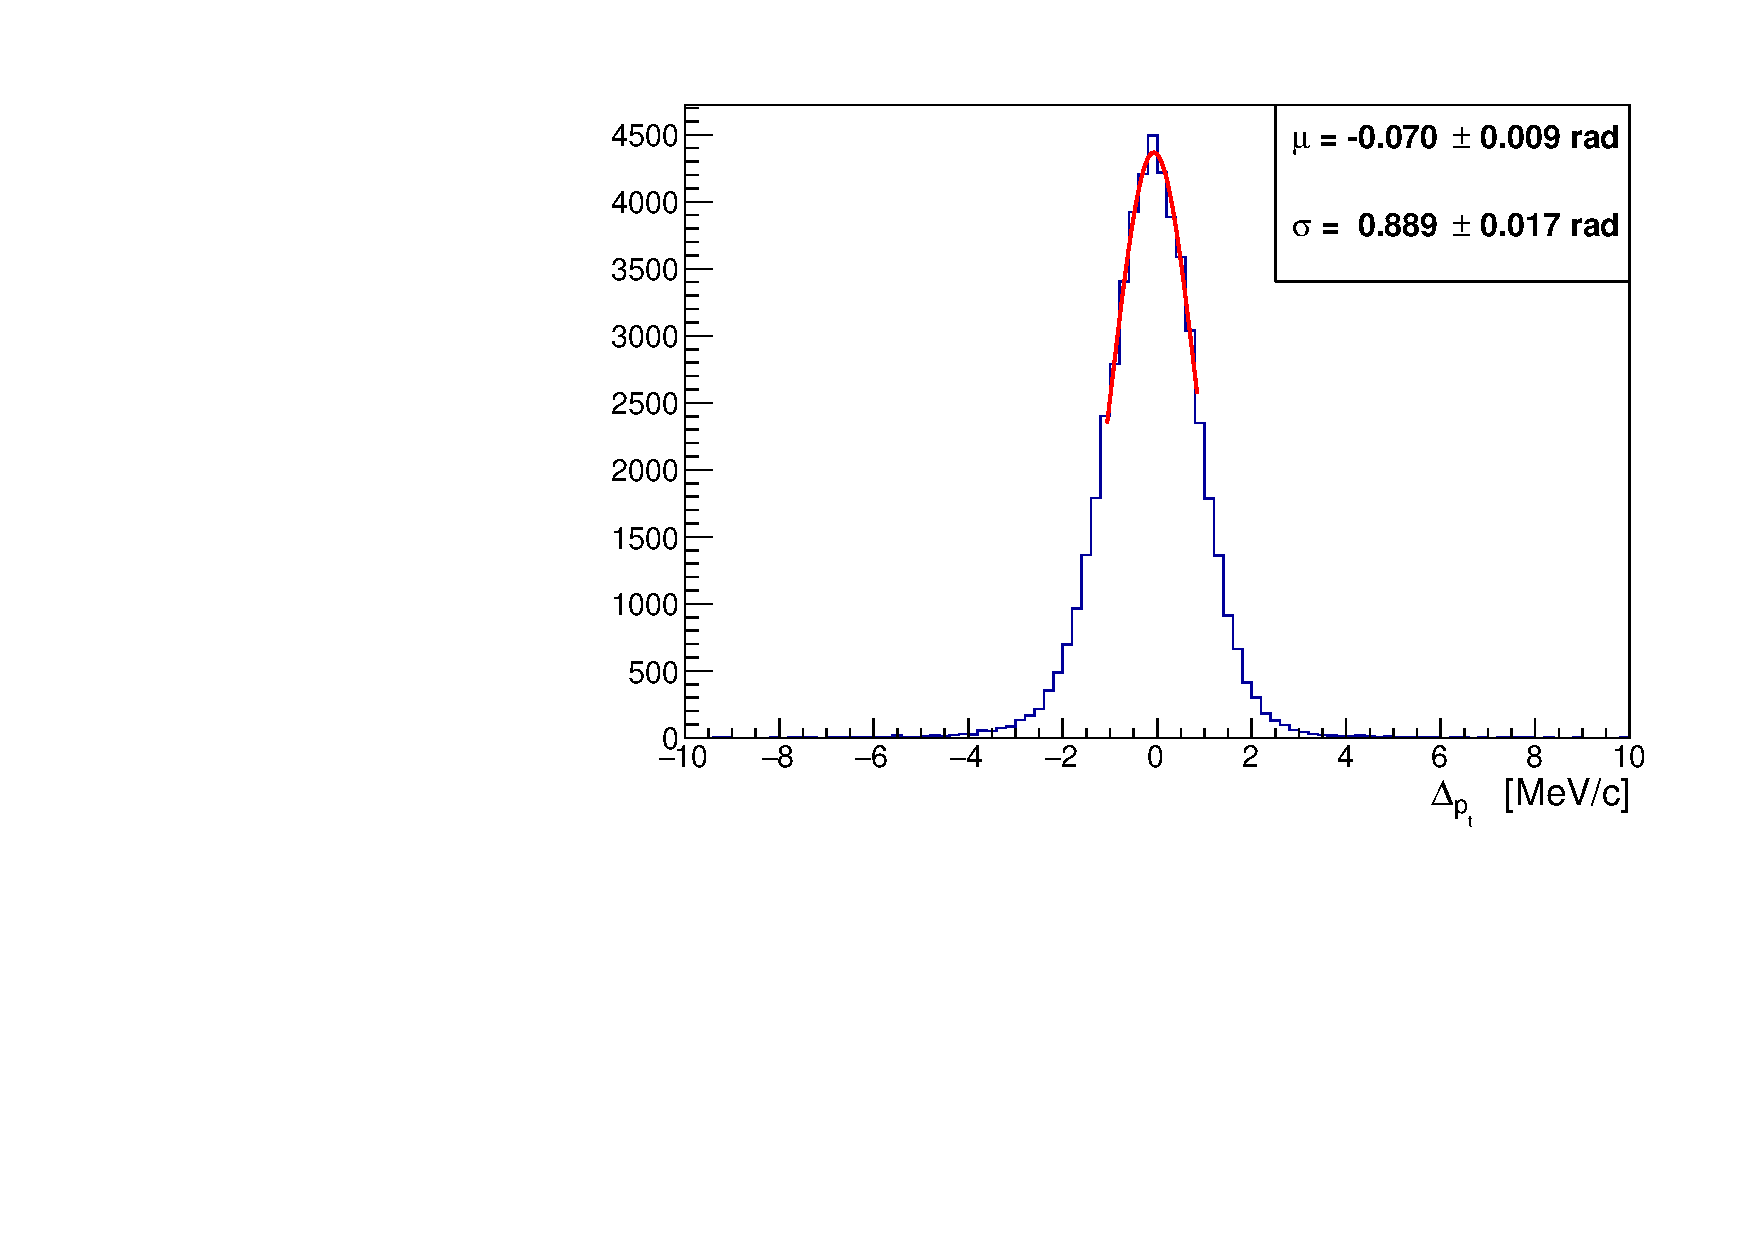
\includegraphics[width=0.49\textwidth, angle=0]{08-Performance/upstream_pt_residual.pdf}
      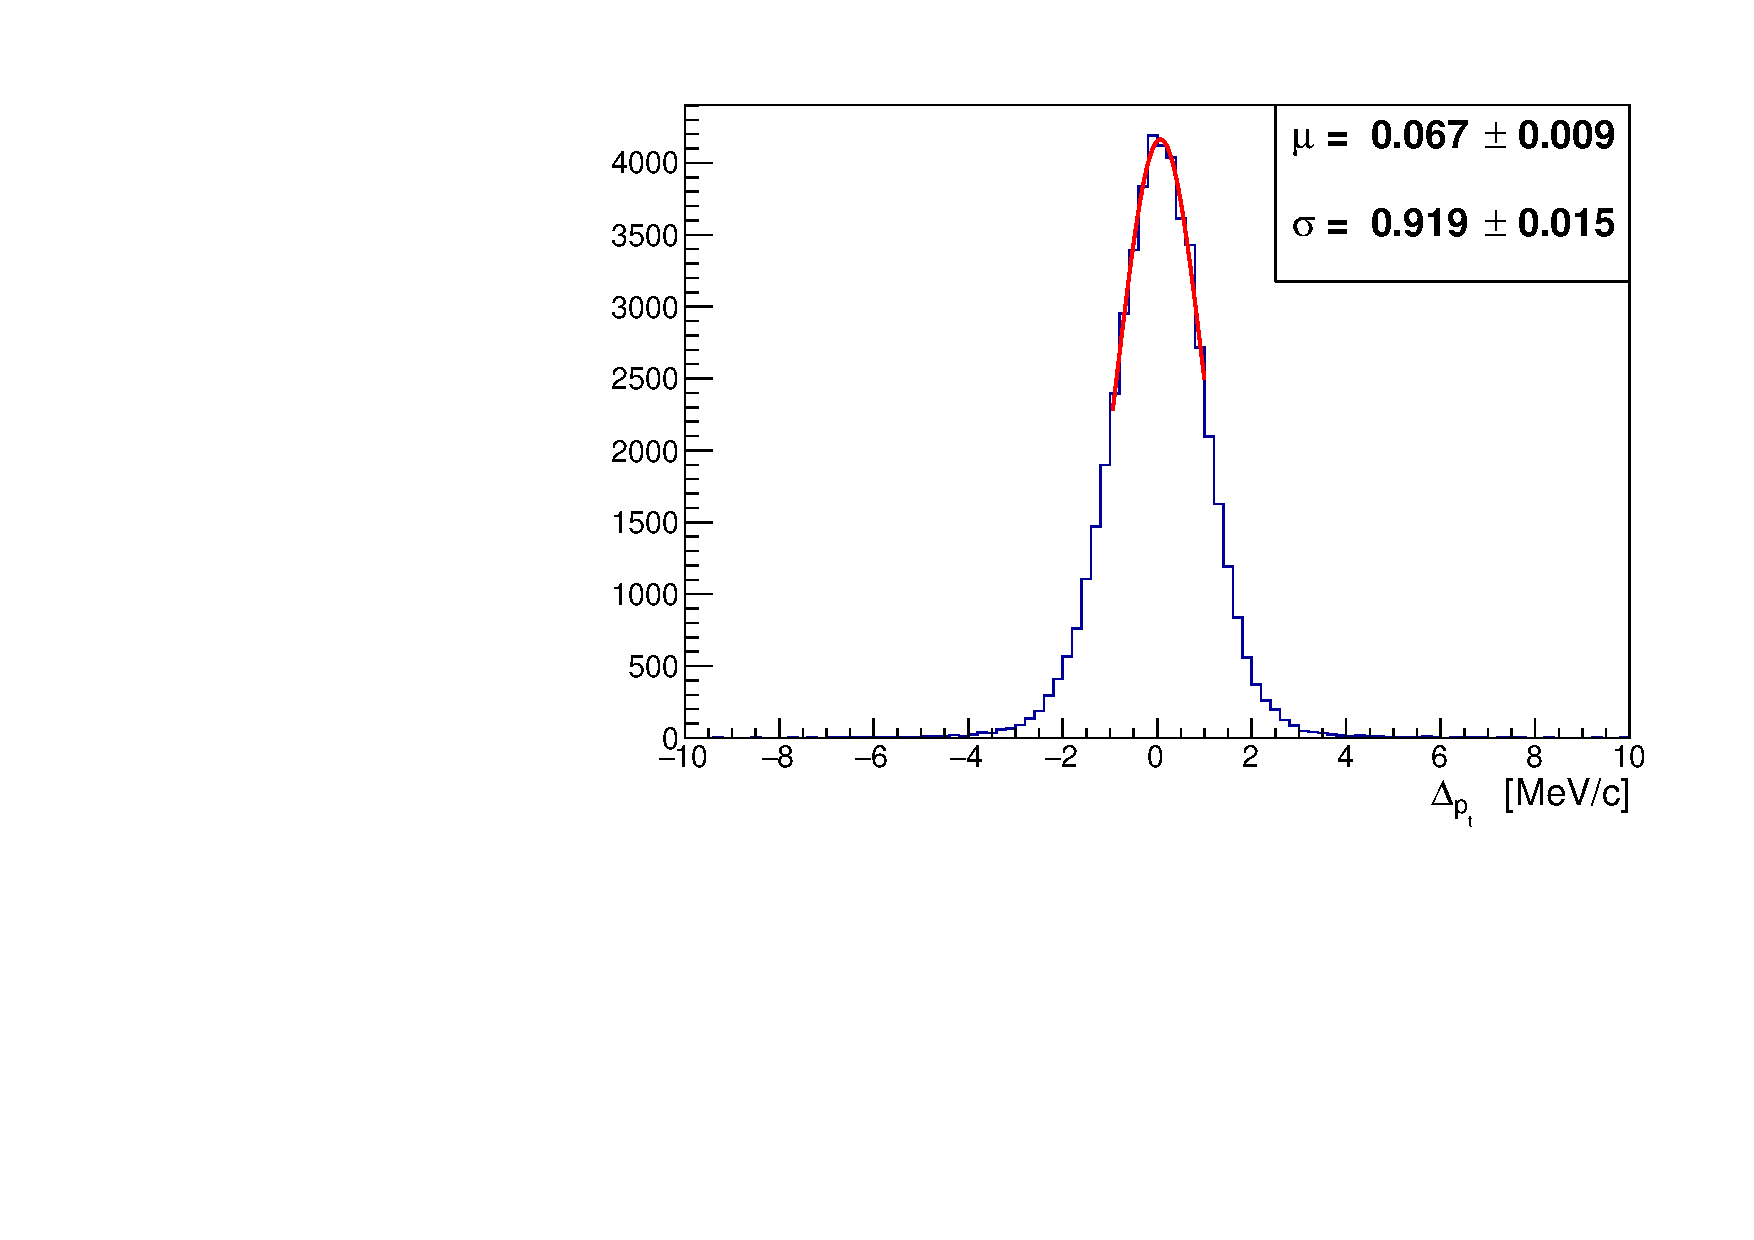
\includegraphics[width=0.49\textwidth, angle=0]{08-Performance/downstream_pt_residual.pdf}
      \caption{\label{fig:PtResidKalman} The $p_{t}$ residuals of the upstream (left) and downstream (right) trackers.}
    \end{center}
  \end{figure}
  
   \begin{figure}[p]
    \begin{center}
      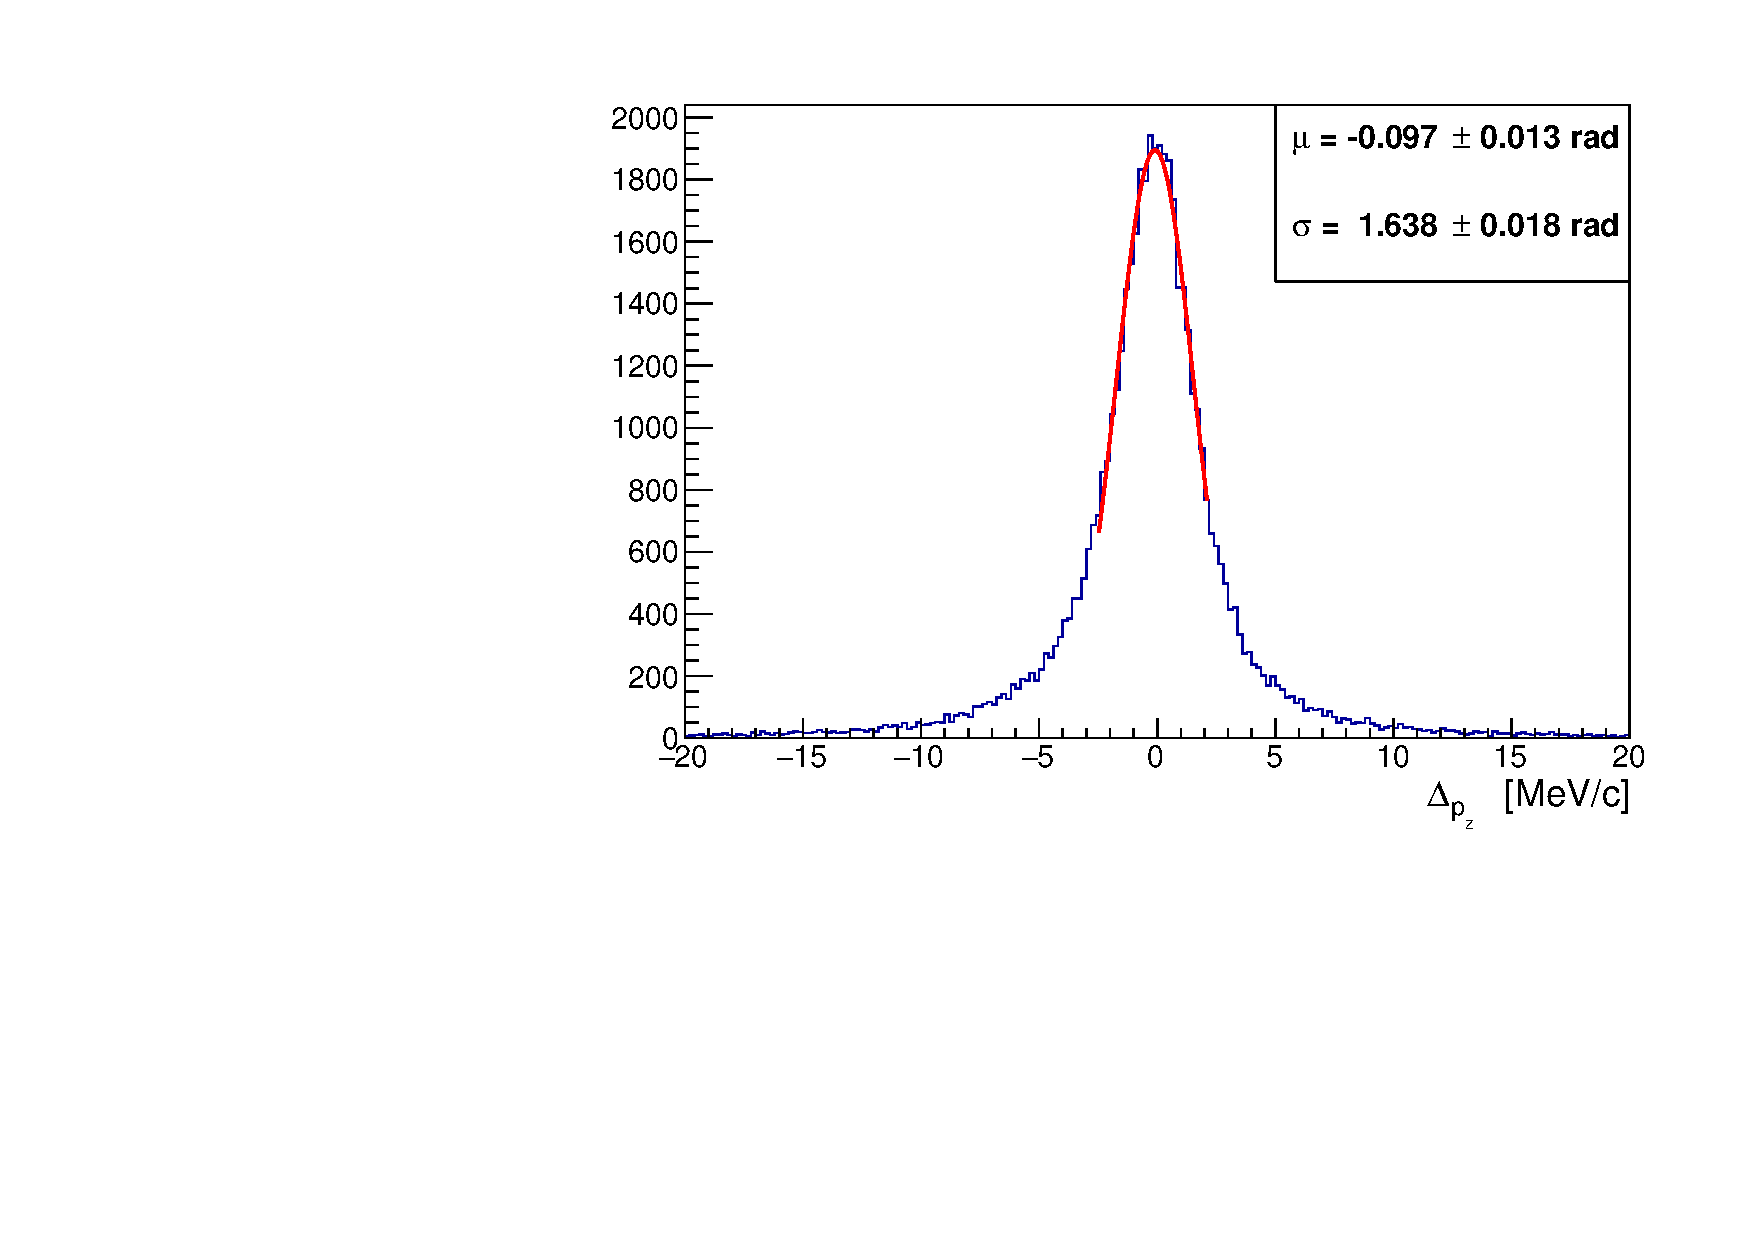
\includegraphics[width=0.49\textwidth, angle=0]{08-Performance/upstream_pz_residual.pdf}
      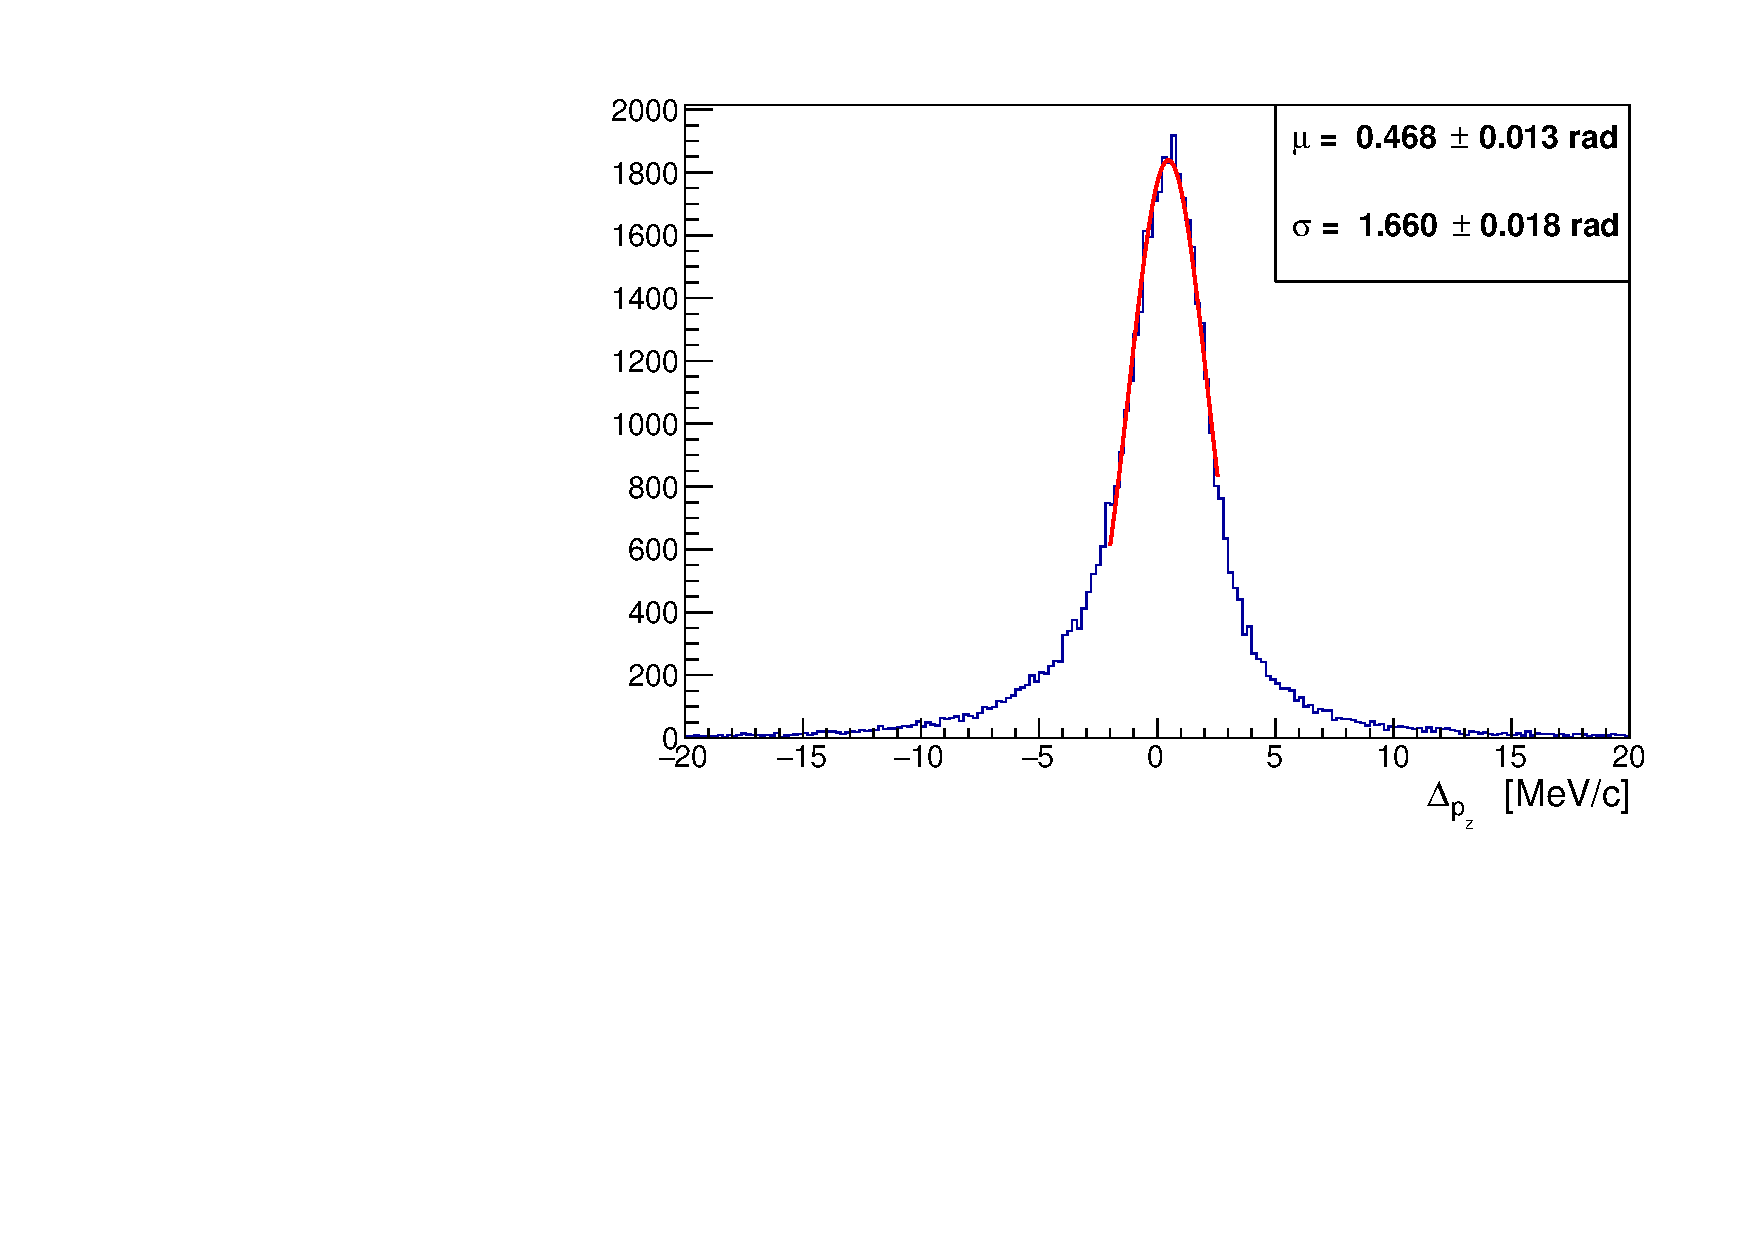
\includegraphics[width=0.49\textwidth, angle=0]{08-Performance/downstream_pz_residual.pdf}
      \caption{\label{fig:PzResidKalman} The $p_z$ residuals of the upstream (left) and downstream (right) trackers.}
    \end{center}
  \end{figure}
  
%   \begin{figure}[p]
%     \begin{center}
%       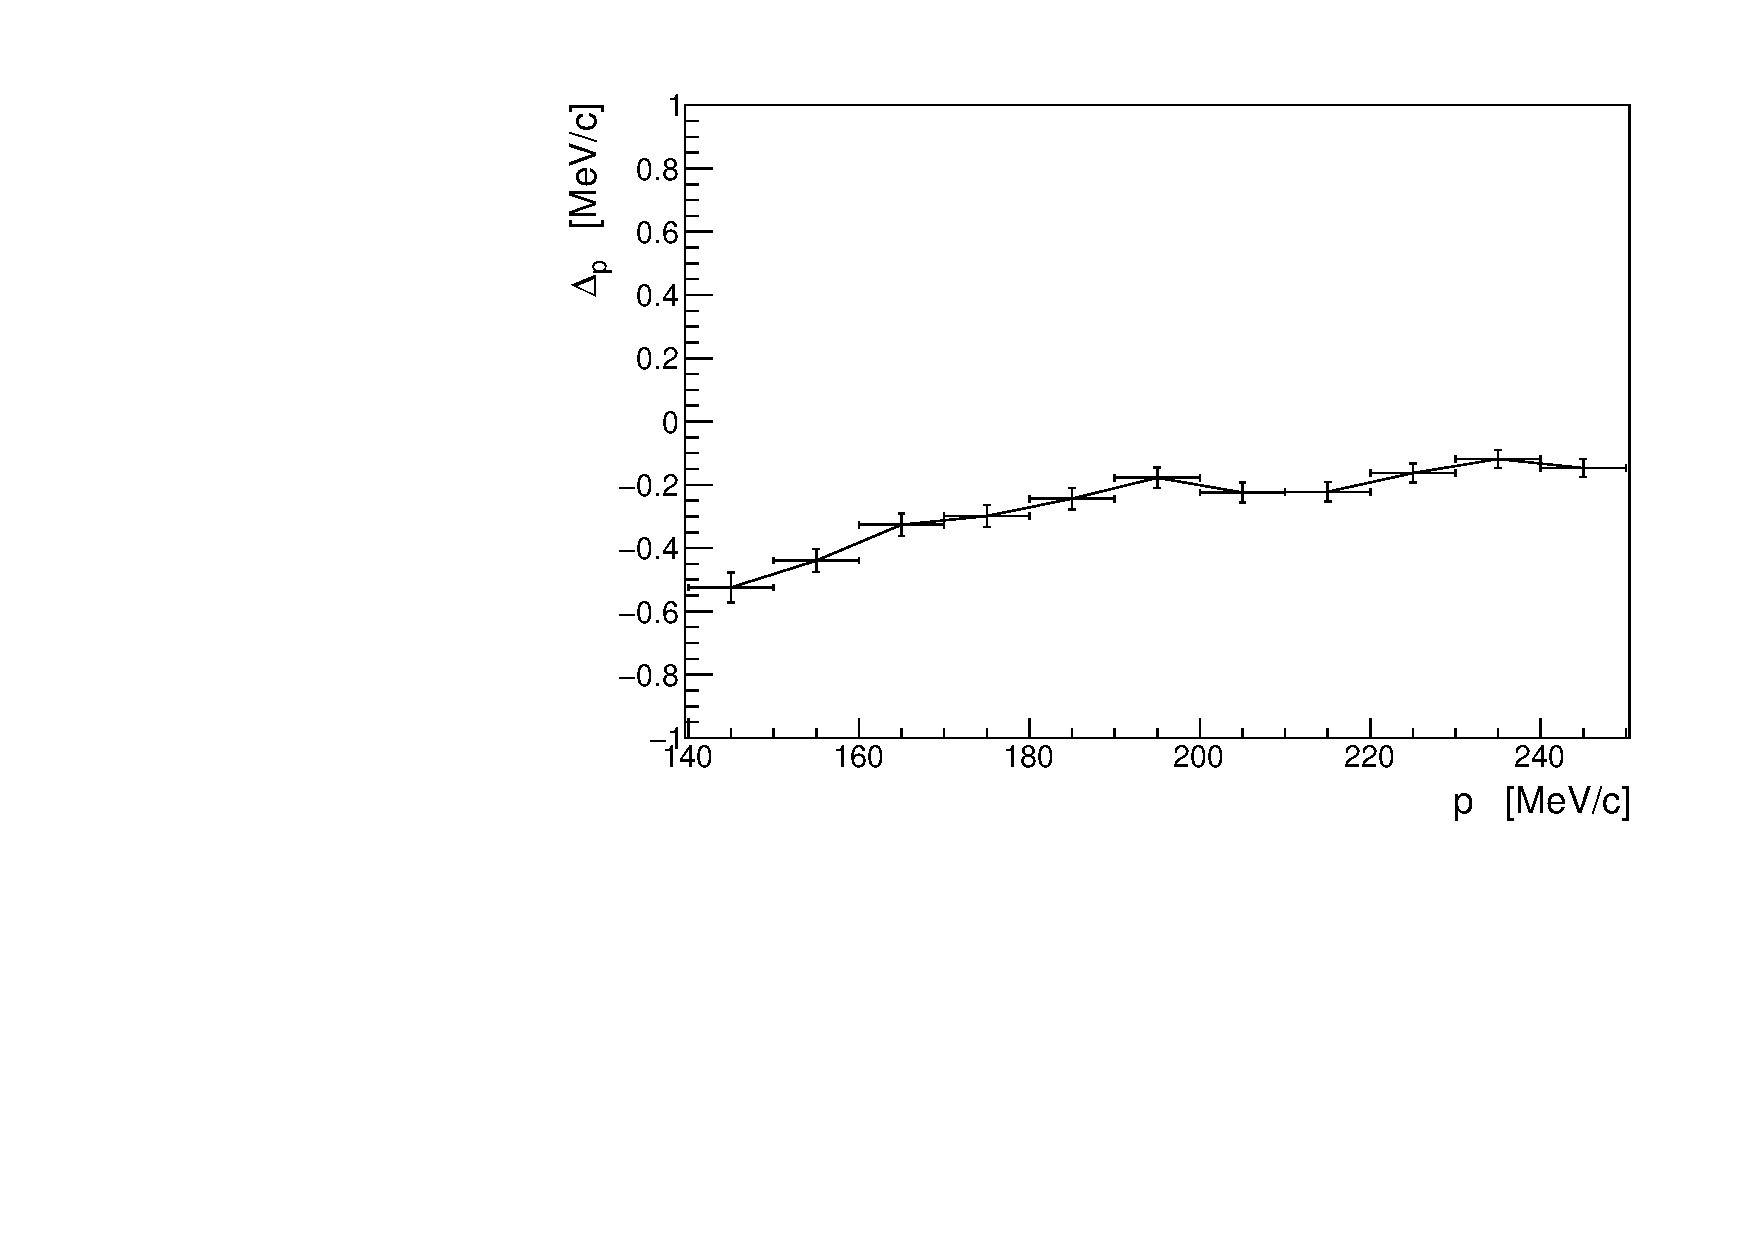
\includegraphics[width=0.49\textwidth, angle=0]{08-Performance/upstream_p_bias_p.pdf}
%       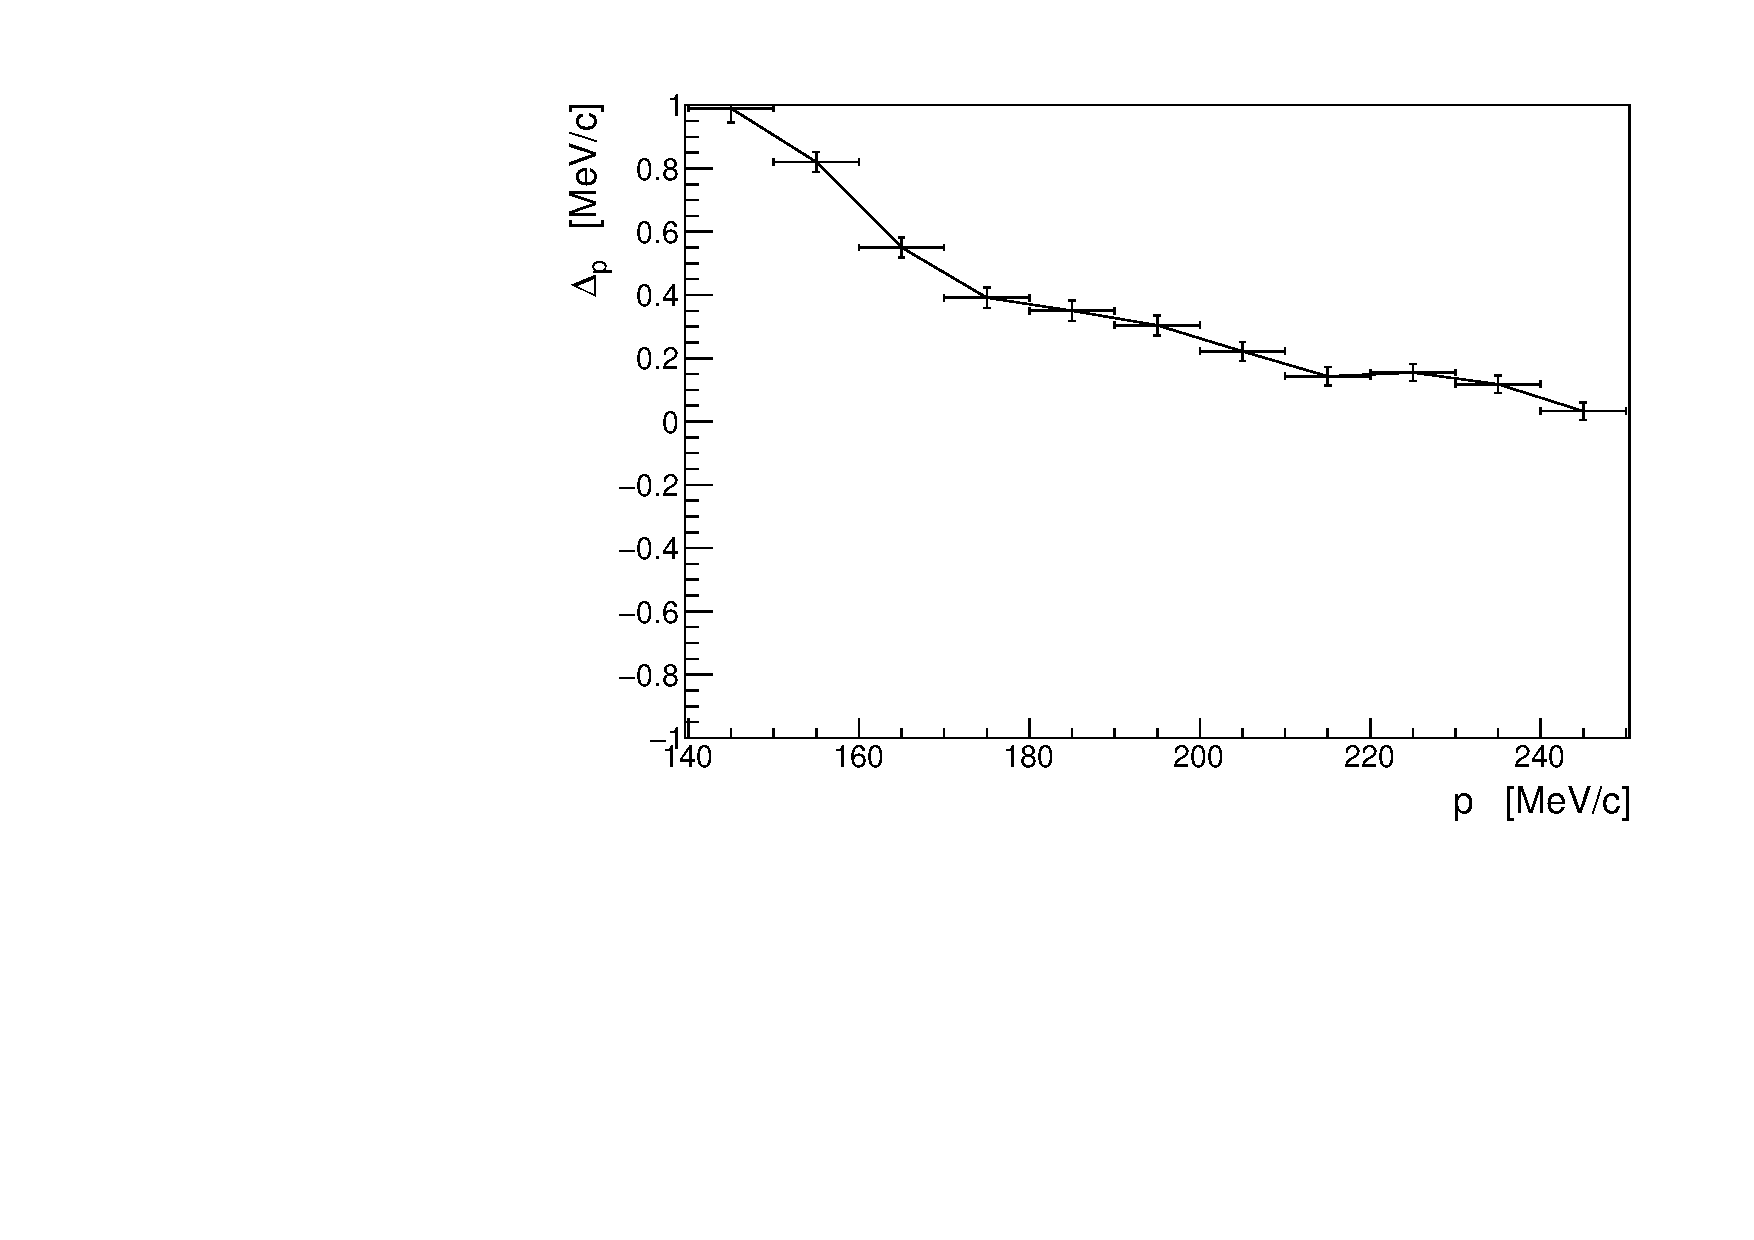
\includegraphics[width=0.49\textwidth, angle=0]{08-Performance/downstream_p_bias_p.pdf}
%       \caption{\label{fig:pBiasKalman} The mean residual between the final track fit total momentum and the true track momentum, evaluated at the reference plane.}
%     \end{center}
%   \end{figure}
  
  \begin{figure}[p]
   \begin{center}
     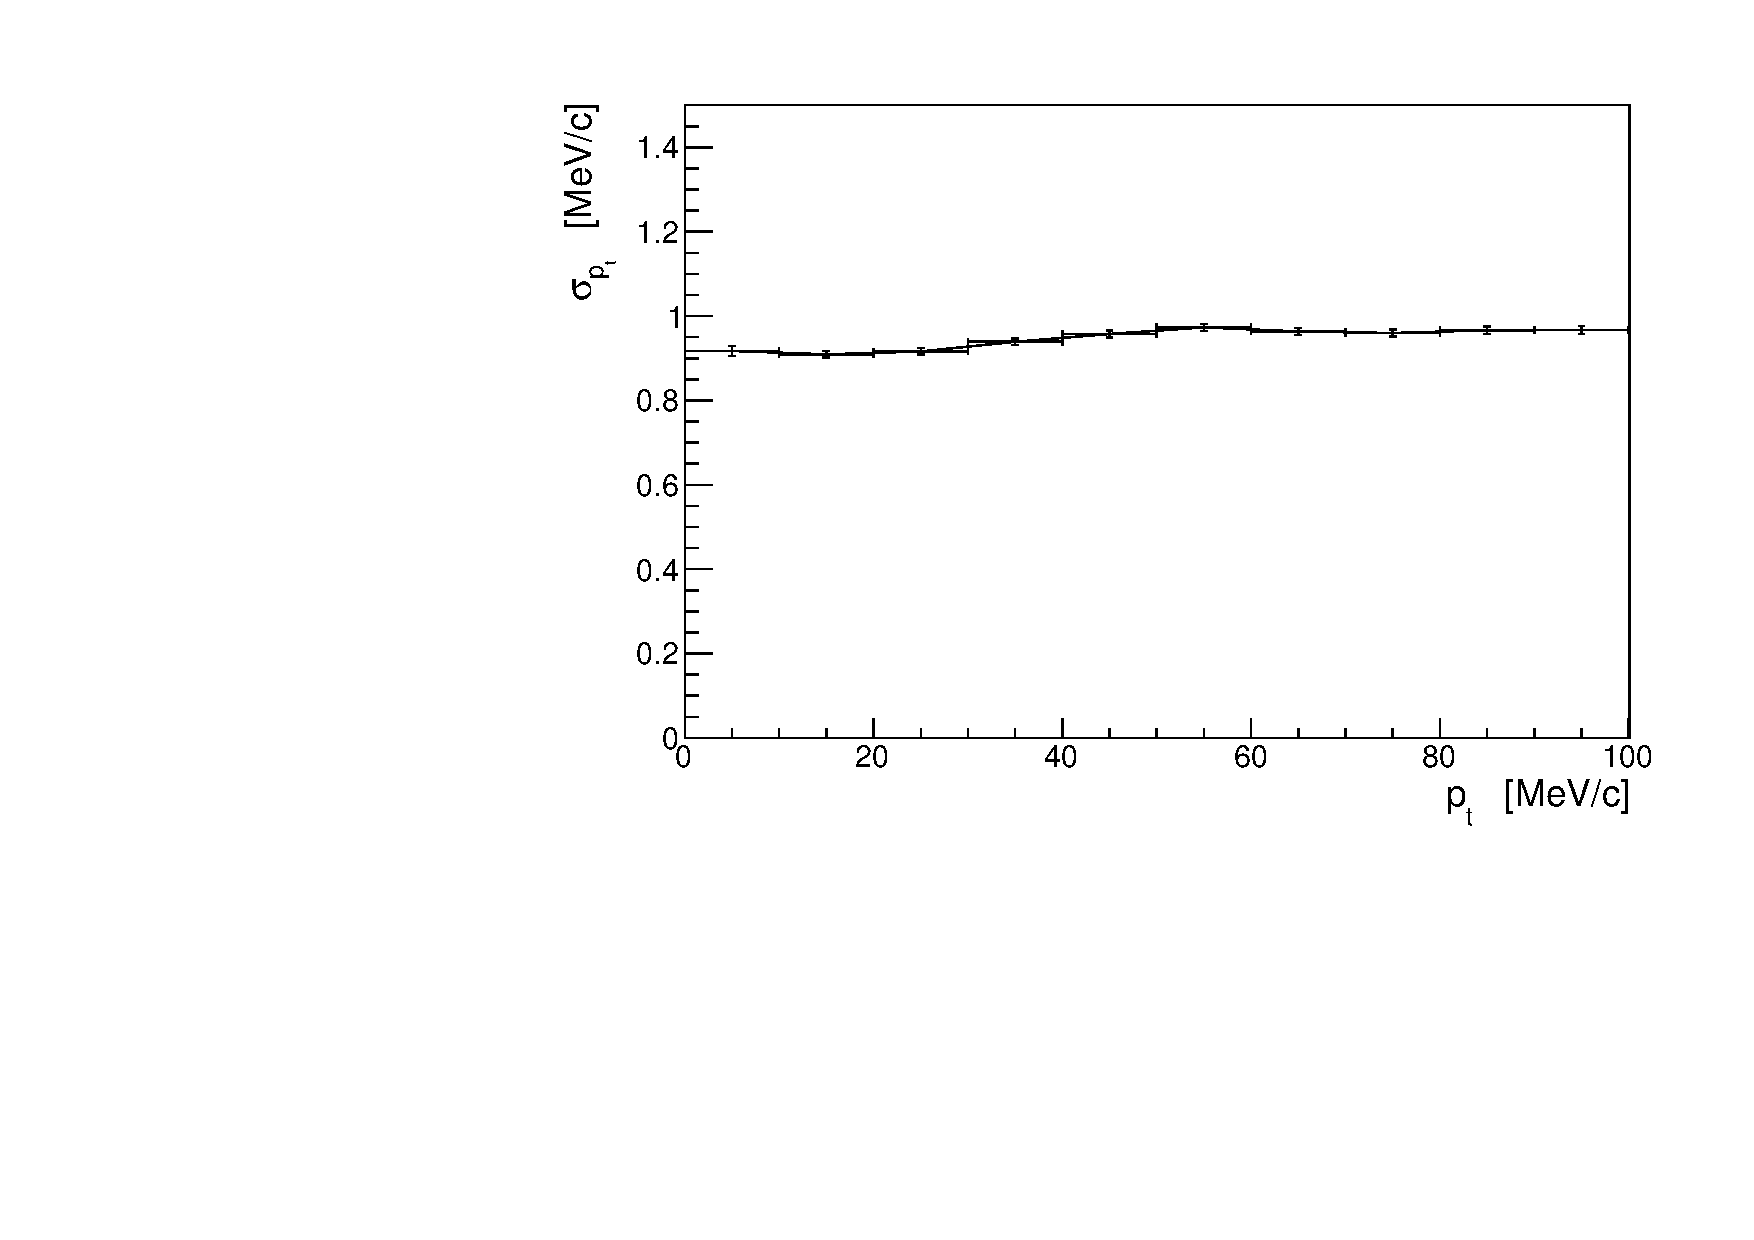
\includegraphics[width=0.49\textwidth, angle=0]{08-Performance/upstream_pt_resolution_pt.pdf}
     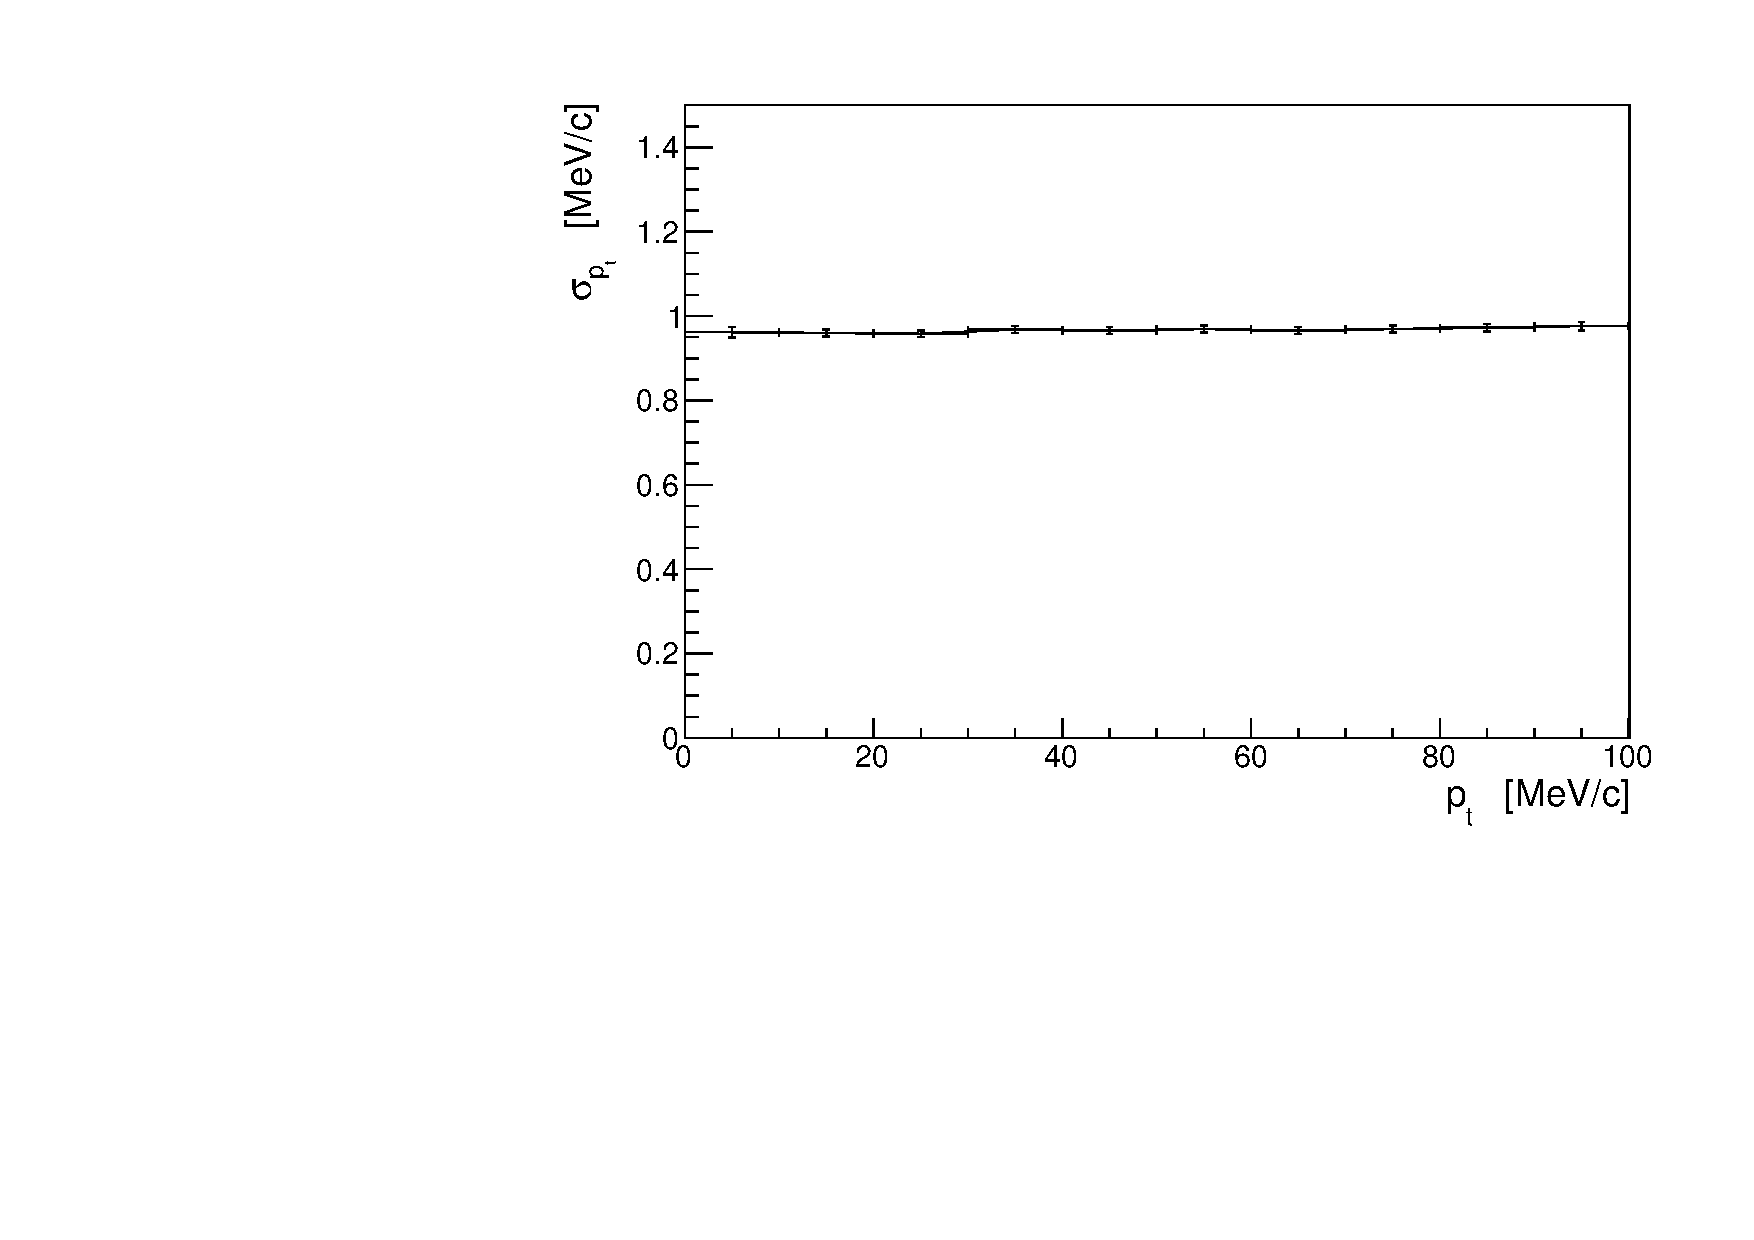
\includegraphics[width=0.49\textwidth, angle=0]{08-Performance/downstream_pt_resolution_pt.pdf}
     \caption{\label{fig:PtPtResolKalman} The $p_{t}$ resolution as a function of the $p_{t}$ of the upstream (left) and downstream (right) trackers.}
   \end{center}
  \end{figure}
  
  \begin{figure}[p]
   \begin{center}
     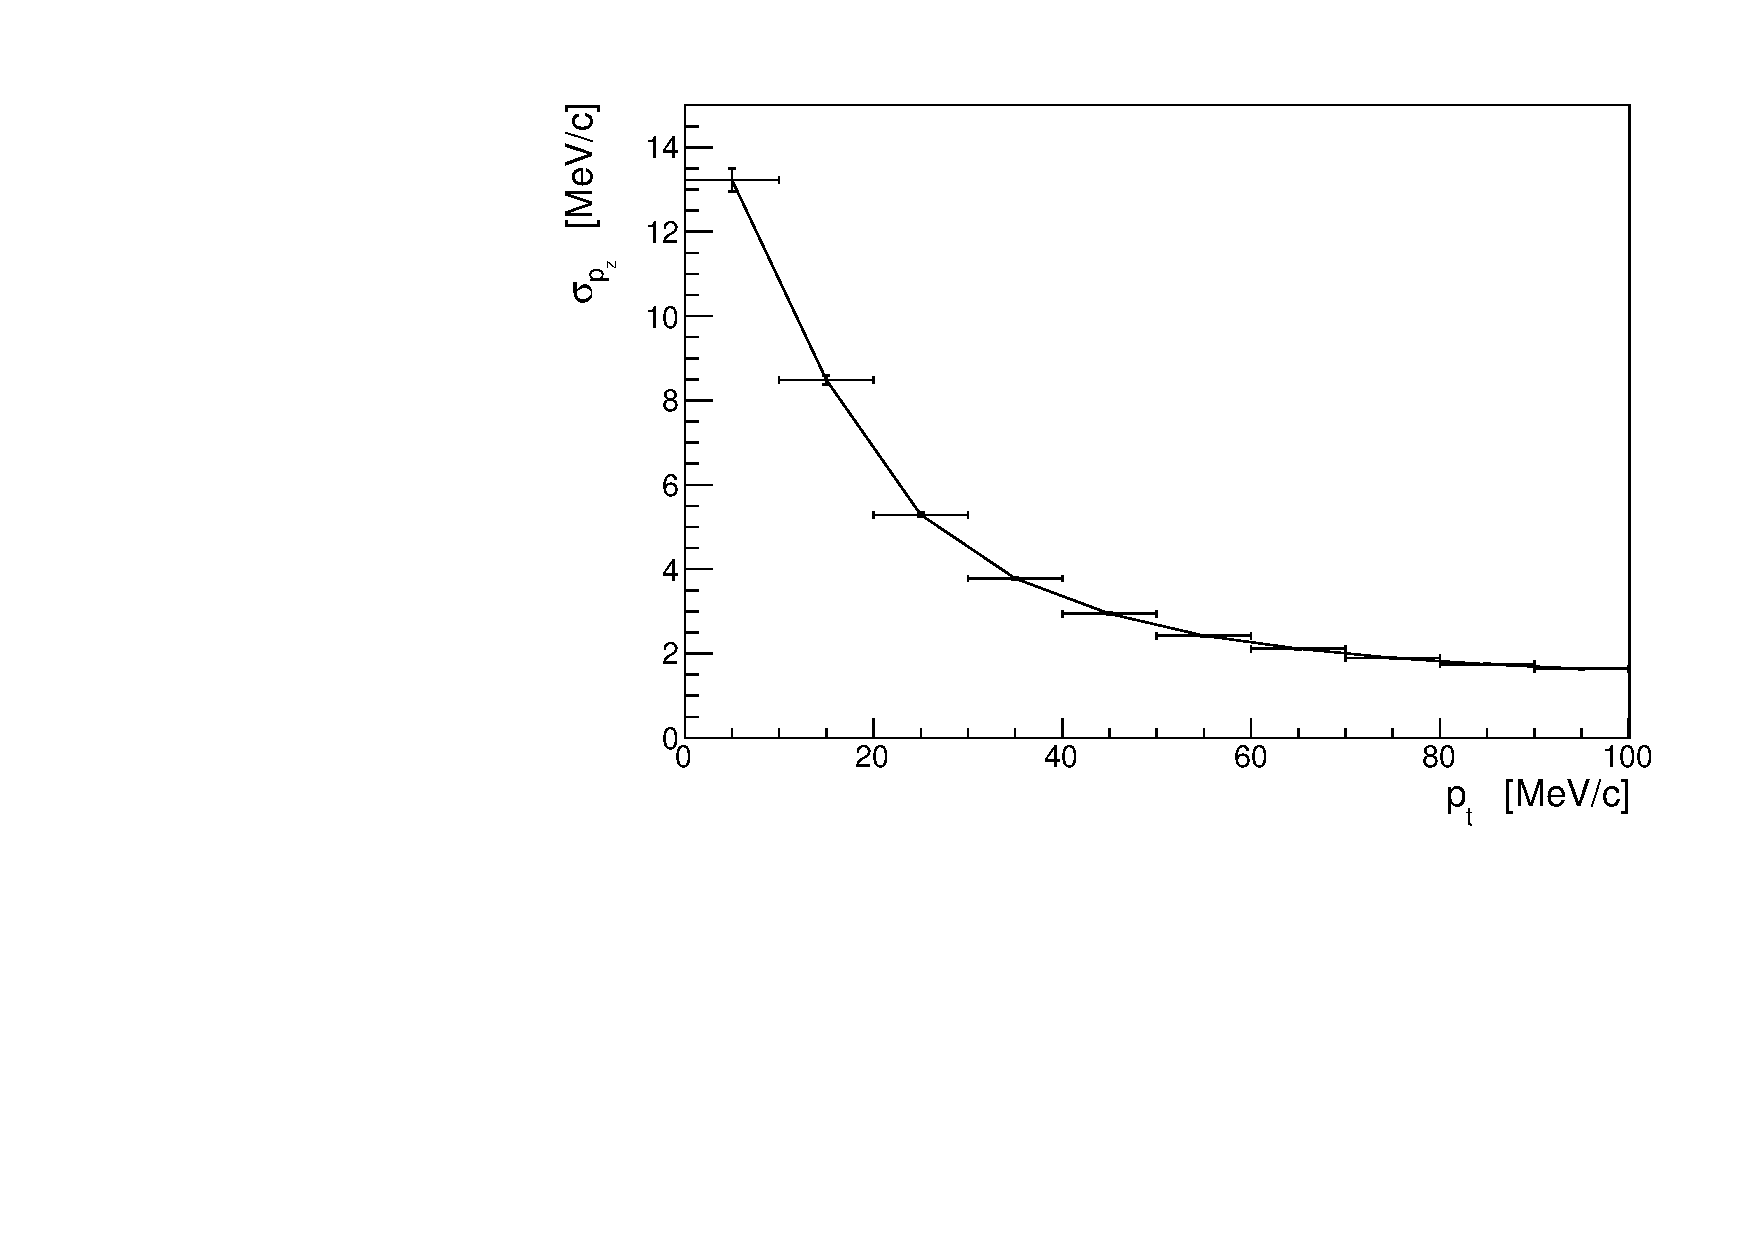
\includegraphics[width=0.49\textwidth, angle=0]{08-Performance/upstream_pz_resolution_pt.pdf}
     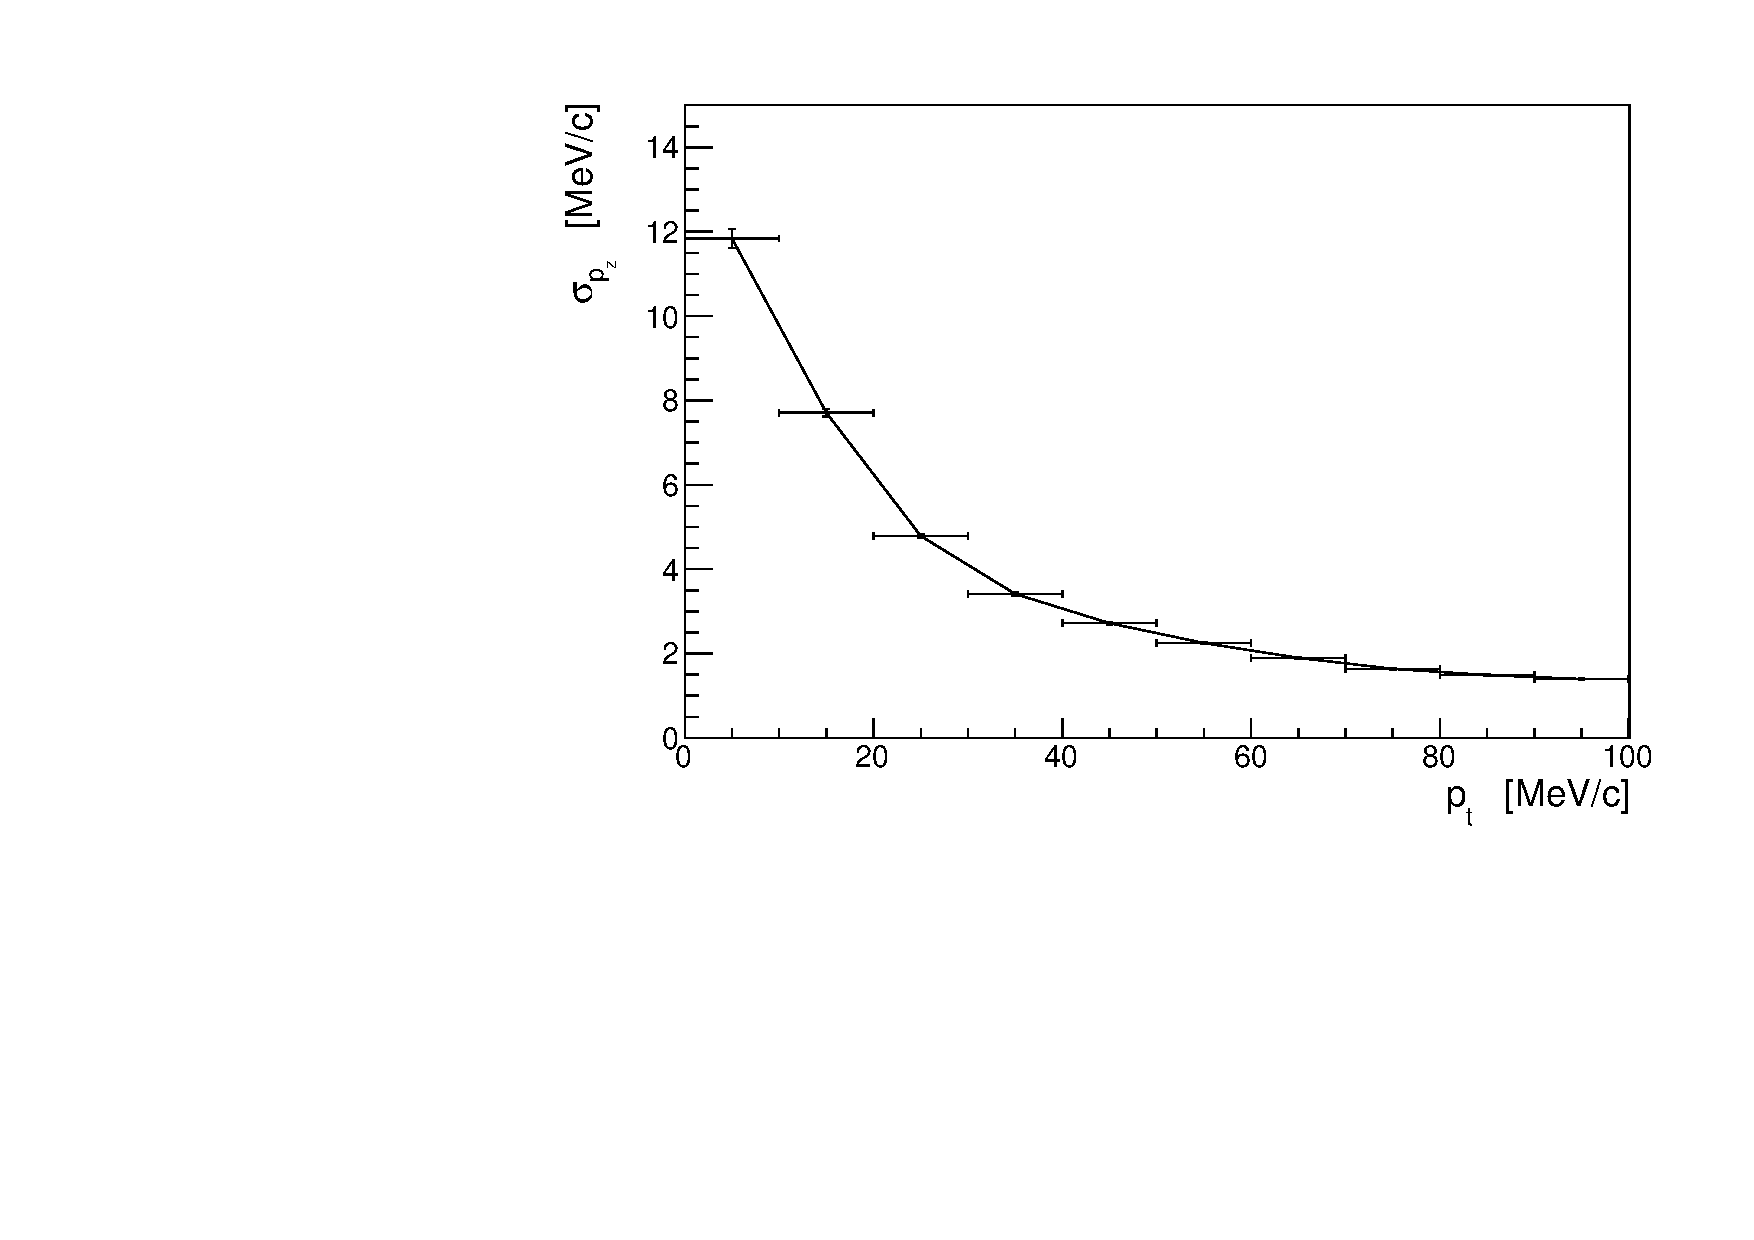
\includegraphics[width=0.49\textwidth, angle=0]{08-Performance/downstream_pz_resolution_pt.pdf}
     \caption{\label{fig:PtPzResolKalman} The $p_z$ resolution vs the $p_{t}$ of the upstream (left) and downstream (right) trackers.}
   \end{center}
  \end{figure}
